% ============================================================
%  编译原理期中大作业实验报告
%  类Rust语言词法分析与语法分析器设计与实现
%  作者：程浩然、黄艺鑫
% ============================================================

\documentclass[12pt,a4paper]{ctexart}

% 页面设置
\usepackage[top=2.5cm, bottom=2.5cm, left=2.5cm, right=2.5cm]{geometry}

% 基础宏包
\usepackage{amsmath, amssymb}
\usepackage{graphicx}
\usepackage{xcolor}
\usepackage{hyperref}
\usepackage{booktabs}
\usepackage{longtable}
\usepackage{float}
\usepackage{multirow}
\usepackage{array}

% 代码高亮
\usepackage{listings}
\lstset{
    basicstyle=\ttfamily\small,
    keywordstyle=\color{blue}\bfseries,
    commentstyle=\color{gray}\itshape,
    stringstyle=\color{red},
    numbers=left,
    numberstyle=\tiny\color{gray},
    numbersep=5pt,
    frame=single,
    breaklines=true,
    breakatwhitespace=true,
    tabsize=4,
    showstringspaces=false,
    captionpos=b
}

% 定义语言样式
\lstdefinelanguage{RustLike}{
    keywords={fn, let, mut, if, else, while, for, in, loop, break, continue, return, i32},
    morekeywords=[2]{Program, Function, Block, LetStmt, IfStmt, WhileStmt, ForStmt, LoopStmt, ReturnStmt},
    keywordstyle=[2]\color{purple},
    sensitive=true,
    morecomment=[l]{//},
    morecomment=[s]{/*}{*/},
    morestring=[b]",
    morestring=[b]',
}

\lstdefinelanguage{Flex}{
    keywords={DIGIT, NoneZeroDigit, OctalDigit, HexadecimalDigit, BinaryDigit, Chars, Identifier, IntegerConstant, FloatingConstant, StringConst, CharacterConstant},
    sensitive=true,
    morecomment=[l]{//},
    morecomment=[s]{/*}{*/},
}


% 段落间距
\setlength{\parskip}{0.5em}

% 超链接样式
\hypersetup{
    colorlinks=true,
    linkcolor=blue,
    urlcolor=blue,
    citecolor=blue
}

% 标题信息
\title{\textbf{编译原理期中大作业实验报告}\\[0.5em]
\large 类Rust语言词法分析与语法分析器设计与实现}
\author{
    \begin{tabular}{rl}
        学院：& 计算机科学与技术学院 \\
        专业：& 计算机科学与技术 \\
        学号：& 2351579 / 2253797 / 2352628 \\
        姓名：& 程浩然 / 黄艺鑫 / 韦畅 \\
        指导教师：& 高珍、卫志华 \\
        学期：& 2026 年春季学期
    \end{tabular}
}
\date{\today}

\begin{document}

% ============================================================
%  封面
% ============================================================
\begin{titlepage}
\centering
\vspace*{\fill}

{\LARGE\textbf{编译原理期中大作业实验报告}\\[1em]
\large 类Rust语言词法分析与语法分析器设计与实现}

\vspace{3em}

{\renewcommand{\arraystretch}{1.8}
\begin{tabular}{rl}
    学院：& 计算机科学与技术学院 \\
    专业：& 计算机科学与技术 \\
    学号：& 2351579 / 2253797 / 2352628 \\
    姓名：& 程浩然 / 黄艺鑫 / 韦畅 \\
    指导教师：& 高珍、卫志华 \\
    学期：& 2026 年春季学期
\end{tabular}
}

\vspace{2em}
{\today}

\vspace*{\fill}
\end{titlepage}

% ============================================================
%  目录
% ============================================================
\tableofcontents
\newpage

% ============================================================
%  摘要
% ============================================================
\section*{摘要}
\addcontentsline{toc}{section}{摘要}

本项目实现了一个针对类Rust语言的前端编译器，包含完整的词法分析器和语法分析器模块。词法分析器使用Flex工具实现，能够识别关键字、运算符、常量、标识符等多种词法单元；语法分析器采用递归下降分析法，能够解析函数定义、变量声明、控制流语句和各类表达式结构。此外，项目还基于ImGui框架实现了图形化界面，支持词法单元流和语法树的可视化展示。

本报告详细阐述了目标语言的文法定义、词法分析与语法分析的理论基础、各模块的具体设计与实现方案，并通过完整的测试用例验证了系统的正确性。项目采用CMake构建系统，支持Linux和Windows双平台编译运行。

\textbf{关键词：}词法分析、语法分析、递归下降、Flex、编译原理、类Rust语言

\newpage

% ============================================================
%  第一章 概述
% ============================================================
\section{概述}

\subsection{项目背景与目标}

编译原理是计算机科学的核心课程之一，它系统性地介绍了从源代码到目标代码的完整转换过程。本次期中大作业旨在通过实践加深对编译器前端——词法分析与语法分析的理解，掌握相关理论与实现技术。

本项目的核心目标是：
\begin{enumerate}
    \item 设计并实现一个完整的词法分析器，能够将源代码字符串转换为词法单元序列
    \item 设计并实现一个语法分析器，能够将词法单元序列转换为语法树
    \item 理解并应用词法分析（有限状态自动机）和语法分析（递归下降）的理论基础
    \item 实现图形化界面，提供直观的分析结果展示
\end{enumerate}

\subsection{目标语言简介}

本项目选择类Rust语言作为目标语言，主要基于以下考量：

\begin{enumerate}
    \item \textbf{语法简洁}：Rust语言语法结构清晰，既保留了现代语言特性，又避免了过于复杂的语法规则
    \item \textbf{类型明确}：Rust强调显式类型声明，便于语法分析时处理类型信息
    \item \textbf{学习价值}：Rust作为新兴编程语言，了解其语法特点对未来技术发展有参考意义
\end{enumerate}

本项目支持的类Rust语言特性包括：
\begin{itemize}
    \item 函数定义与调用
    \item 变量声明（支持\texttt{mut}可变修饰符）
    \item 基础数据类型（\texttt{i32}、\texttt{bool}等）
    \item 数组类型与数组操作
    \item 控制流语句（\texttt{if-else}、\texttt{while}、\texttt{for-in}、\texttt{loop}）
    \item 表达式（算术运算、比较运算、范围表达式）
    \item 注释（行注释、块注释）
\end{itemize}

\subsection{团队分工与开发环境}

\begin{table}[H]
\centering
\caption{团队分工表}
\begin{tabular}{|c|c|l|}
\hline
\textbf{姓名} & \textbf{学号} & \textbf{主要分工} \\
\hline
程浩然 & 2351579 & 词法分析器设计与实现（Flex 规则编写、Token 体系设计）、 \\
 & & 词法-语法接口对接、GUI 可视化模块、跨平台构建系统 \\
\hline
黄艺鑫 & 2253797 & 语法分析器设计与实现（递归下降解析器）、语法树数据结构设计、 \\
 & & 表达式优先级处理、CLI 命令行接口 \\
\hline
韦畅 & 2352628 & 实验报告撰写、测试用例设计与验证、文法规则整理与分析 \\
\hline
\end{tabular}
\end{table}

\begin{table}[H]
\centering
\caption{开发环境配置}
\begin{tabular}{|l|l|}
\hline
\textbf{组件} & \textbf{版本/说明} \\
\hline
操作系统 & Linux (Ubuntu) / Windows 11 \\
\hline
编译器 & GCC/G++ (Linux), MinGW-w64 (Windows) \\
\hline
Flex版本 & 2.6.4 \\
\hline
CMake版本 & 3.10+ \\
\hline
GUI框架 & ImGui + GLFW + OpenGL3 \\
\hline
构建工具链 & vcpkg（依赖管理） \\
\hline
\end{tabular}
\end{table}

\subsection{系统架构}

\begin{figure}[H]
    \centering
    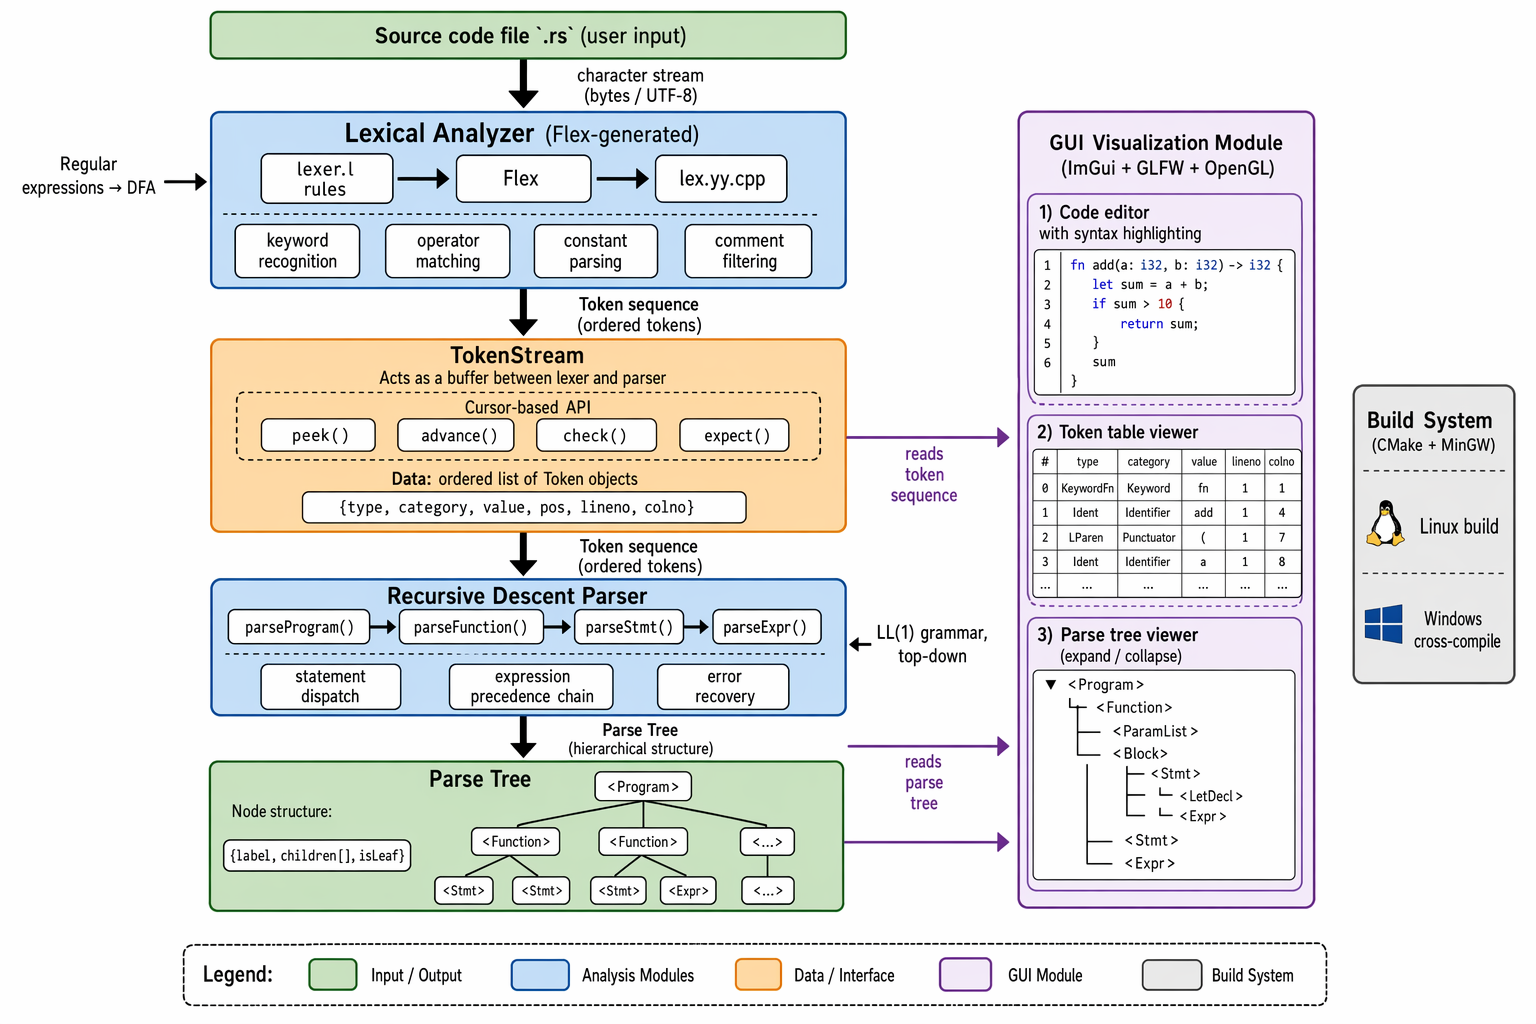
\includegraphics[width=\textwidth]{figures/system_architecture.png}
    \caption{系统总体架构图}
\end{figure}

系统由以下核心模块组成：

\begin{enumerate}
    \item \textbf{词法分析器}：负责将源代码字符串分解为词法单元（Token）
    \item \textbf{语法分析器}：负责将Token序列组织为语法树
    \item \textbf{TokenStream}：作为词法分析器与语法分析器之间的接口
    \item \textbf{GUI模块}：提供图形化界面，展示分析结果
    \item \textbf{构建系统}：管理编译过程，支持跨平台构建
\end{enumerate}

\newpage

% ============================================================
%  第二章 目标语言文法定义
% ============================================================
\section{目标语言文法定义}

文法是描述语言语法结构的形式化方法，是编译器设计的基础。本章详细定义目标语言的词法规则和语法规则。

\subsection{词法规则}

词法规则定义了源代码中可以被识别的最小单位——词法单元（Token）。本项目将Token分为以下几类：

\subsubsection{关键字}

关键字是语言中具有特殊含义的保留词，不能作为标识符使用。

\begin{longtable}{|l|l|l|}
\caption{关键字定义表} \label{tab:keywords} \\
\hline
\textbf{关键字} & \textbf{种别码} & \textbf{功能说明} \\
\hline
\endfirsthead
\hline
\textbf{关键字} & \textbf{种别码} & \textbf{功能说明} \\
\hline
\endhead
\hline
\endfoot
\hline
\endlastfoot

\texttt{let} & Let & 变量声明 \\
\texttt{mut} & Mut & 可变修饰符 \\
\texttt{fn} & Fn & 函数定义 \\
\texttt{if} & If & 条件分支 \\
\texttt{else} & Else & 否则分支 \\
\texttt{while} & While & 当型循环 \\
\texttt{for} & For & 遍历循环 \\
\texttt{in} & In & 范围迭代 \\
\texttt{loop} & Loop & 无限循环 \\
\texttt{break} & Break & 跳出循环 \\
\texttt{continue} & Continue & 继续循环 \\
\texttt{return} & Return & 函数返回 \\
\end{longtable}

\subsubsection{运算符}

运算符用于执行各种计算和比较操作。

\begin{longtable}{|l|l|l|}
\caption{运算符定义表} \label{tab:operators} \\
\hline
\textbf{运算符} & \textbf{种别码} & \textbf{功能说明} \\
\hline
\endfirsthead
\hline
\textbf{运算符} & \textbf{种别码} & \textbf{功能说明} \\
\hline
\endhead
\hline
\endfoot
\hline
\endlastfoot

\texttt{->} & Arrow & 返回类型声明 \\
\texttt{..} & DotDot & 范围运算符 \\
\texttt{.} & Dot & 成员访问 \\
\texttt{==} & EqualEqual & 相等比较 \\
\texttt{!=} & NotEqual & 不等比较 \\
\texttt{>=} & GreaterEqual & 大于等于 \\
\texttt{<=} & LessEqual & 小于等于 \\
\texttt{>} & Greater & 大于 \\
\texttt{<} & Less & 小于 \\
\texttt{+} & Plus & 加法 \\
\texttt{-} & Minus & 减法 \\
\texttt{*} & Star & 乘法/解引用 \\
\texttt{/} & Slash & 除法 \\
\texttt{\&} & Ampersand & 引用/位运算 \\
\end{longtable}

\subsubsection{界符}

界符用于分隔和组织语法结构。

\begin{longtable}{|l|l|l|}
\caption{界符定义表} \label{tab:delimiters} \\
\hline
\textbf{界符} & \textbf{种别码} & \textbf{功能说明} \\
\hline
\endfirsthead
\hline
\textbf{界符} & \textbf{种别码} & \textbf{功能说明} \\
\hline
\endhead
\hline
\endfoot
\hline
\endlastfoot

\texttt{=} & Assign & 赋值 \\
\texttt{;} & Semicolon & 语句结束 \\
\texttt{:} & Colon & 类型声明 \\
\texttt{,} & Comma & 参数分隔 \\
\texttt{(} & LParen & 左圆括号 \\
\texttt{)} & RParen & 右圆括号 \\
\texttt{\{} & LBrace & 左花括号 \\
\texttt{\}} & RBrace & 右花括号 \\
\texttt{[} & LBracket & 左方括号 \\
\texttt{]} & RBracket & 右方括号 \\
\texttt{\#} & End & 程序结束标记 \\
\end{longtable}

\subsubsection{常量类型}

常量是程序中的固定值，本项目支持四种常量类型：

\begin{table}[H]
\centering
\caption{常量类型定义}
\begin{tabular}{|l|l|l|}
\hline
\textbf{常量类型} & \textbf{种别码} & \textbf{示例} \\
\hline
整数常量 & IntegerConstant & \texttt{42}, \texttt{0xFF}, \texttt{0b1010} \\
\hline
浮点常量 & FloatingConstant & \texttt{3.14}, \texttt{2.5e10} \\
\hline
字符串常量 & StringConst & \texttt{"hello"} \\
\hline
字符常量 & CharacterConstant & \texttt{'a'}, \texttt{'\textbackslash n'} \\
\hline
\end{tabular}
\end{table}

\subsubsection{标识符与类型声明符}

\begin{table}[H]
\centering
\caption{标识符与类型声明符}
\begin{tabular}{|l|l|l|}
\hline
\textbf{类型} & \textbf{种别码} & \textbf{说明} \\
\hline
标识符 & Identifier & 以字母或下划线开头，后跟字母、数字或下划线 \\
\hline
类型声明符 & Declerator & 如 \texttt{i32} \\
\hline
\end{tabular}
\end{table}

\subsubsection{注释}

\begin{table}[H]
\centering
\caption{注释类型}
\begin{tabular}{|l|l|l|}
\hline
\textbf{注释类型} & \textbf{种别码} & \textbf{格式} \\
\hline
行注释 & LineComment & \texttt{//} 开头，至行尾 \\
\hline
块注释 & BlockComment & \texttt{/* */} 包围 \\
\hline
\end{tabular}
\end{table}

\subsection{语法规则}

本节按作业要求的编号体系（0.1--9.3）逐条列出文法产生式。作业明确要求完成的必选规则为 0.1--0.3、1.1--1.5、2.0--2.2、3.1--3.5、4.1、5.0--5.1，其余为扩展规则。每条规则标注实现状态：\textcolor{green!60!black}{\textbf{[已实现]}} 或 \textcolor{red!70!black}{\textbf{[未实现]}}，必选规则额外注明"必选"。

% ============================================================
%  基础定义
% ============================================================
\subsubsection{基础定义（规则 0.1 -- 0.3）}

\textbf{规则 0.1\quad 变量属性} \hfill \textcolor{green!60!black}{\textbf{[已实现 · 必选]}}

\begin{align}
\langle\text{变量属性}\rangle &\rightarrow \texttt{mut}
\end{align}

变量属性用于修饰可变变量。实现中通过 \texttt{ts.check("Mut")} 判断是否存在 \texttt{mut} 关键字。

\textbf{规则 0.2\quad 类型} \hfill \textcolor{green!60!black}{\textbf{[已实现 · 必选]}}

\begin{align}
\langle\text{类型}\rangle &\rightarrow \texttt{i32}
\end{align}

基础类型仅包含 \texttt{i32}，在词法分析器中以种别码 \texttt{I32}（类型为 \texttt{declerator}）识别。后续扩展规则将增加数组类型、引用类型、元组类型等形式。

\textbf{规则 0.3\quad 左值} \hfill \textcolor{green!60!black}{\textbf{[已实现 · 必选]}}

\begin{align}
\langle\text{左值}\rangle &\rightarrow \langle\text{可取引用}\rangle \\
\langle\text{可取引用}\rangle &\rightarrow \langle\text{可取元素}\rangle \\
\langle\text{可取元素}\rangle &\rightarrow \texttt{ID}
\end{align}

左值的处理采用统一策略：先调用 \texttt{parseExpr()} 解析表达式，再检查是否跟随赋值号 \texttt{=}，从而区分赋值语句与表达式语句。后续扩展规则为 $\langle\text{可取引用}\rangle$ 和 $\langle\text{可取元素}\rangle$ 添加更多候选产生式。

% ============================================================
%  程序结构
% ============================================================
\subsubsection{程序结构（规则 1.1 -- 1.5）}

\textbf{规则 1.1\quad 基础程序} \hfill \textcolor{green!60!black}{\textbf{[已实现 · 必选]}}

\begin{align}
Program &\rightarrow \langle\text{声明串}\rangle \\
\langle\text{声明串}\rangle &\rightarrow \epsilon \mid \langle\text{声明}\rangle \ \langle\text{声明串}\rangle \\
\langle\text{声明}\rangle &\rightarrow \langle\text{函数声明}\rangle \\
\langle\text{函数声明}\rangle &\rightarrow \langle\text{函数头声明}\rangle \ \langle\text{语句块}\rangle \\
\langle\text{函数头声明}\rangle &\rightarrow \texttt{fn} \ \texttt{ID} \ \texttt{(} \ \langle\text{形参列表}\rangle \ \texttt{)} \\
\langle\text{形参列表}\rangle &\rightarrow \epsilon \\
\langle\text{语句块}\rangle &\rightarrow \texttt{\{} \ \langle\text{语句串}\rangle \ \texttt{\}} \\
\langle\text{语句串}\rangle &\rightarrow \epsilon
\end{align}

\textbf{规则 1.2\quad 语句}（拓展 1.1） \hfill \textcolor{green!60!black}{\textbf{[已实现 · 必选]}}

\begin{align}
\langle\text{语句串}\rangle &\rightarrow \langle\text{语句}\rangle \ \langle\text{语句串}\rangle \\
\langle\text{语句}\rangle &\rightarrow \texttt{;}
\end{align}

在 \texttt{parseStmt()} 中，若当前 Token 为 \texttt{Semicolon}，则创建 \texttt{EmptyStmt} 节点。

\textbf{规则 1.3\quad 返回语句}（拓展 1.2） \hfill \textcolor{green!60!black}{\textbf{[已实现 · 必选]}}

\begin{align}
\langle\text{语句}\rangle &\rightarrow \langle\text{返回语句}\rangle \\
\langle\text{返回语句}\rangle &\rightarrow \texttt{return} \ \texttt{;}
\end{align}

在 \texttt{parseReturnStmt()} 中，若 \texttt{return} 后直接是分号，则不解析表达式。

\textbf{规则 1.4\quad 函数输入}（依赖 0.1、0.2，拓展 1.1） \hfill \textcolor{green!60!black}{\textbf{[已实现 · 必选]}}

\begin{align}
\langle\text{形参列表}\rangle &\rightarrow \langle\text{形参}\rangle \mid \langle\text{形参}\rangle \ \texttt{,} \ \langle\text{形参列表}\rangle \\
\langle\text{形参}\rangle &\rightarrow \langle\text{变量属性}\rangle \ \texttt{ID} \ \texttt{:} \ \langle\text{类型}\rangle
\end{align}

由 \texttt{parseParamList()} 和 \texttt{parseParam()} 实现。若当前符号为 \texttt{RParen} 则选择 $\epsilon$，否则解析形参并以逗号为分隔循环解析。

\textbf{规则 1.5\quad 函数输出}（依赖 0.2、3.1，拓展 1.1、1.3） \hfill \textcolor{green!60!black}{\textbf{[已实现 · 必选]}}

\begin{align}
\langle\text{函数头声明}\rangle &\rightarrow \texttt{fn} \ \texttt{ID} \ \texttt{(} \ \langle\text{形参列表}\rangle \ \texttt{)} \ \texttt{->} \ \langle\text{类型}\rangle \\
\langle\text{返回语句}\rangle &\rightarrow \texttt{return} \ \langle\text{表达式}\rangle \ \texttt{;}
\end{align}

在 \texttt{parseFuncHeader()} 中，若 \texttt{RParen} 后检测到 \texttt{Arrow}（\texttt{->}）则继续解析返回类型。

% ============================================================
%  变量声明与赋值
% ============================================================
\subsubsection{变量声明与赋值（规则 2.0 -- 2.3）}

\textbf{规则 2.0\quad 变量声明}（依赖 0.1、0.2） \hfill \textcolor{green!60!black}{\textbf{[已实现 · 必选]}}

\begin{align}
\langle\text{变量声明}\rangle &\rightarrow \langle\text{变量属性}\rangle \ \texttt{ID} \\
\langle\text{变量声明}\rangle &\rightarrow \langle\text{变量属性}\rangle \ \texttt{ID} \ \texttt{:} \ \langle\text{类型}\rangle
\end{align}

在 \texttt{parseLetStmt()} 中创建 \texttt{VarDecl} 子节点，可选地解析 \texttt{mut}、标识符和类型注解。

\textbf{规则 2.1\quad 变量声明语句}（依赖 2.0，拓展 1.2） \hfill \textcolor{green!60!black}{\textbf{[已实现 · 必选]}}

\begin{align}
\langle\text{语句}\rangle &\rightarrow \langle\text{变量声明语句}\rangle \\
\langle\text{变量声明语句}\rangle &\rightarrow \texttt{let} \ \langle\text{变量声明}\rangle \ \texttt{;}
\end{align}

\textbf{规则 2.2\quad 赋值语句}（依赖 0.3、3.1，拓展 1.2） \hfill \textcolor{green!60!black}{\textbf{[已实现 · 必选]}}

\begin{align}
\langle\text{语句}\rangle &\rightarrow \langle\text{赋值语句}\rangle \\
\langle\text{赋值语句}\rangle &\rightarrow \langle\text{左值}\rangle \ \texttt{=} \ \langle\text{表达式}\rangle \ \texttt{;}
\end{align}

由 \texttt{parseExprOrAssignStmt()} 实现：先解析表达式作为左部，若后跟 \texttt{=} 则构造赋值语句节点，否则构造表达式语句节点。

\textbf{规则 2.3\quad 变量声明赋值语句}（依赖 2.0、3.1，拓展 1.2） \hfill \textcolor{green!60!black}{\textbf{[已实现 · 扩展]}}

\begin{align}
\langle\text{语句}\rangle &\rightarrow \langle\text{变量声明赋值语句}\rangle \\
\langle\text{变量声明赋值语句}\rangle &\rightarrow \texttt{let} \ \langle\text{变量声明}\rangle \ \texttt{=} \ \langle\text{表达式}\rangle \ \texttt{;}
\end{align}

在 \texttt{parseLetStmt()} 中，变量声明后若检测到 \texttt{Assign}（\texttt{=}）则继续解析初始化表达式。

% ============================================================
%  表达式
% ============================================================
\subsubsection{表达式（规则 3.1 -- 3.5）}

表达式文法原始形式存在左递归，不利于递归下降分析。以下给出消除左递归后的等价形式。

\textbf{规则 3.1\quad 基本表达式}（依赖 0.3，拓展 1.2） \hfill \textcolor{green!60!black}{\textbf{[已实现 · 必选]}}

\begin{align}
\langle\text{语句}\rangle &\rightarrow \langle\text{表达式}\rangle \ \texttt{;} \\
\langle\text{表达式}\rangle &\rightarrow \langle\text{加减表达式}\rangle \\
\langle\text{加减表达式}\rangle &\rightarrow \langle\text{项}\rangle \\
\langle\text{项}\rangle &\rightarrow \langle\text{因子}\rangle \\
\langle\text{因子}\rangle &\rightarrow \texttt{NUM} \mid \langle\text{左值}\rangle \mid \texttt{(} \ \langle\text{表达式}\rangle \ \texttt{)}
\end{align}

\textbf{规则 3.2\quad 增加比较运算}（依赖 3.1，拓展 3.1） \hfill \textcolor{green!60!black}{\textbf{[已实现 · 必选]}}

\begin{align}
\langle\text{表达式}\rangle &\rightarrow \langle\text{表达式}\rangle \ \langle\text{比较运算符}\rangle \ \langle\text{加减表达式}\rangle \\
\langle\text{比较运算符}\rangle &\rightarrow \texttt{<} \mid \texttt{<=} \mid \texttt{>} \mid \texttt{>=} \mid \texttt{==} \mid \texttt{!=}
\end{align}

由 \texttt{parseCmpExpr()} 实现，使用循环结构处理连续的比较运算。

\textbf{规则 3.3\quad 增加加减运算}（依赖 3.1，拓展 3.1） \hfill \textcolor{green!60!black}{\textbf{[已实现 · 必选]}}

\begin{align}
\langle\text{加减表达式}\rangle &\rightarrow \langle\text{加减表达式}\rangle \ \langle\text{加减运算符}\rangle \ \langle\text{项}\rangle \\
\langle\text{加减运算符}\rangle &\rightarrow \texttt{+} \mid \texttt{-}
\end{align}

由 \texttt{parseAddExpr()} 实现。

\textbf{规则 3.4\quad 增加乘除运算}（依赖 3.1，拓展 3.1） \hfill \textcolor{green!60!black}{\textbf{[已实现 · 必选]}}

\begin{align}
\langle\text{项}\rangle &\rightarrow \langle\text{项}\rangle \ \langle\text{乘除运算符}\rangle \ \langle\text{因子}\rangle \\
\langle\text{乘除运算符}\rangle &\rightarrow \texttt{*} \mid \texttt{/}
\end{align}

由 \texttt{parseTerm()} 实现。

\textbf{规则 3.5\quad 增加函数调用}（依赖 3.1，拓展 3.1） \hfill \textcolor{green!60!black}{\textbf{[已实现 · 必选]}}

\begin{align}
\langle\text{因子}\rangle &\rightarrow \texttt{ID} \ \texttt{(} \ \langle\text{实参列表}\rangle \ \texttt{)} \\
\langle\text{实参列表}\rangle &\rightarrow \epsilon \mid \langle\text{表达式}\rangle \mid \langle\text{表达式}\rangle \ \texttt{,} \ \langle\text{实参列表}\rangle
\end{align}

在 \texttt{parseAtom()} 中，若标识符后跟 \texttt{LParen} 则构造 \texttt{CallExpr} 节点。参数列表由 \texttt{parseArgList()} 解析。

\textbf{表达式消除左递归后的完整形式。}上述 3.2--3.4 的原始文法含有左递归，实际实现中采用消除左递归后的等价文法：

\begin{align}
Expr &\rightarrow RangeExpr \\
RangeExpr &\rightarrow CmpExpr \mid CmpExpr \ \texttt{..} \ CmpExpr \\
CmpExpr &\rightarrow AddExpr \mid CmpExpr \ CmpOp \ AddExpr \\
CmpOp &\rightarrow \texttt{==} \mid \texttt{!=} \mid \texttt{>} \mid \texttt{>=} \mid \texttt{<} \mid \texttt{<=} \\
AddExpr &\rightarrow MulExpr \mid AddExpr \ AddOp \ MulExpr \\
AddOp &\rightarrow \texttt{+} \mid \texttt{-} \\
MulExpr &\rightarrow Unary \mid MulExpr \ MulOp \ Unary \\
MulOp &\rightarrow \texttt{*} \mid \texttt{/} \\
Unary &\rightarrow \texttt{\&} \ [\texttt{mut}] \ Unary \mid \texttt{*} \ Unary \mid Atom \\
Atom &\rightarrow Constant \mid \texttt{(} \ Expr \ \texttt{)} \mid ArrayLit \\
     &\quad\mid Identifier \ [CallExpr \mid IndexExpr] \\
CallExpr &\rightarrow \texttt{(} \ ArgList \ \texttt{)} \\
IndexExpr &\rightarrow \texttt{[} \ Expr \ \texttt{]} \\
ArgList &\rightarrow \epsilon \mid Expr \mid Expr \ \texttt{,} \ ArgList \\
ArrayLit &\rightarrow \texttt{[} \ ExprList \ \texttt{]} \\
ExprList &\rightarrow \epsilon \mid Expr \mid Expr \ \texttt{,} \ ExprList
\end{align}

运算符优先级从低到高为：范围 \texttt{..} $\rightarrow$ 比较 $\rightarrow$ 加减 $\rightarrow$ 乘除 $\rightarrow$ 单目 $\rightarrow$ 原子，通过函数调用的嵌套层次保证高优先级运算符先被归约。

% ============================================================
%  选择结构
% ============================================================
\subsubsection{选择结构（规则 4.1 -- 4.3）}

\textbf{规则 4.1\quad 选择结构}（依赖 1.1、3.1，拓展 1.2） \hfill \textcolor{green!60!black}{\textbf{[已实现 · 必选]}}

\begin{align}
\langle\text{语句}\rangle &\rightarrow \langle\text{if语句}\rangle \\
\langle\text{if语句}\rangle &\rightarrow \texttt{if} \ \langle\text{表达式}\rangle \ \langle\text{语句块}\rangle \ \langle\text{else部分}\rangle \\
\langle\text{else部分}\rangle &\rightarrow \epsilon
\end{align}

\textbf{规则 4.2\quad 增加 else}（依赖 1.1，拓展 4.1） \hfill \textcolor{green!60!black}{\textbf{[已实现 · 扩展]}}

\begin{align}
\langle\text{else部分}\rangle &\rightarrow \texttt{else} \ \langle\text{语句块}\rangle
\end{align}

\textbf{规则 4.3\quad 增加 else if}（依赖 1.1，拓展 4.1） \hfill \textcolor{green!60!black}{\textbf{[已实现 · 扩展]}}

\begin{align}
\langle\text{else部分}\rangle &\rightarrow \texttt{else} \ \texttt{if} \ \langle\text{表达式}\rangle \ \langle\text{语句块}\rangle \ \langle\text{else部分}\rangle
\end{align}

由 \texttt{parseIfStmt()} 实现，\texttt{else} 部分通过递归调用 \texttt{parseIfStmt()} 处理 \texttt{else if} 链。

% ============================================================
%  循环结构
% ============================================================
\subsubsection{循环结构（规则 5.0 -- 5.4）}

\textbf{规则 5.0\quad 循环语句}（拓展 1.2） \hfill \textcolor{green!60!black}{\textbf{[已实现 · 必选]}}

\begin{align}
\langle\text{语句}\rangle &\rightarrow \langle\text{循环语句}\rangle
\end{align}

\texttt{parseStmt()} 根据 \texttt{While}、\texttt{For}、\texttt{Loop} 关键字分发到对应解析函数。

\textbf{规则 5.1\quad while 循环}（依赖 1.1、3.1，拓展 5.0） \hfill \textcolor{green!60!black}{\textbf{[已实现 · 必选]}}

\begin{align}
\langle\text{循环语句}\rangle &\rightarrow \langle\text{while语句}\rangle \\
\langle\text{while语句}\rangle &\rightarrow \texttt{while} \ \langle\text{表达式}\rangle \ \langle\text{语句块}\rangle
\end{align}

\textbf{规则 5.2\quad for 循环}（依赖 1.1、2.0、3.1，拓展 5.0） \hfill \textcolor{green!60!black}{\textbf{[已实现 · 扩展]}}

\begin{align}
\langle\text{循环语句}\rangle &\rightarrow \langle\text{for语句}\rangle \\
\langle\text{for语句}\rangle &\rightarrow \texttt{for} \ \langle\text{变量声明}\rangle \ \texttt{in} \ \langle\text{可迭代结构}\rangle \ \langle\text{语句块}\rangle \\
\langle\text{可迭代结构}\rangle &\rightarrow \langle\text{表达式}\rangle \ \texttt{..} \ \langle\text{表达式}\rangle
\end{align}

由 \texttt{parseForStmt()} 实现。范围表达式 \texttt{start..end} 在 \texttt{parseExpr()} 中作为 \texttt{RangeExpr} 节点处理。

\textbf{规则 5.3\quad loop 循环}（依赖 1.1，拓展 5.0） \hfill \textcolor{green!60!black}{\textbf{[已实现 · 扩展]}}

\begin{align}
\langle\text{循环语句}\rangle &\rightarrow \langle\text{loop语句}\rangle \\
\langle\text{loop语句}\rangle &\rightarrow \texttt{loop} \ \langle\text{语句块}\rangle
\end{align}

\textbf{规则 5.4\quad break 和 continue}（拓展 1.2） \hfill \textcolor{green!60!black}{\textbf{[已实现 · 扩展]}}

\begin{align}
\langle\text{语句}\rangle &\rightarrow \texttt{break} \ \texttt{;} \mid \texttt{continue} \ \texttt{;}
\end{align}

% ============================================================
%  引用与借用
% ============================================================
\subsubsection{引用与借用（规则 6.1 -- 6.4）}

\textbf{规则 6.1\quad 变量不可变属性}（拓展 0.1） \hfill \textcolor{green!60!black}{\textbf{[已实现 · 扩展]}}

\begin{align}
\langle\text{变量属性}\rangle &\rightarrow \epsilon
\end{align}

变量属性可以为空，即 \texttt{let a;} 声明不可变变量。实现中 \texttt{mut} 为可选项，不出现时即对应此规则。

\textbf{规则 6.2\quad 不可变引用}（依赖 0.2、0.3，拓展 0.2、0.3） \hfill \textcolor{green!60!black}{\textbf{[已实现 · 扩展]}}

\begin{align}
\langle\text{类型}\rangle &\rightarrow \texttt{\&} \ \langle\text{类型}\rangle \\
\langle\text{可取引用}\rangle &\rightarrow \texttt{\&} \ \langle\text{可取引用}\rangle
\end{align}

在 \texttt{parseType()} 中，若当前符号为 \texttt{Ampersand}（\texttt{\&}）则解析引用类型。在 \texttt{parseUnary()} 中处理取地址表达式。

\textbf{规则 6.3\quad 可变引用}（依赖 0.2、0.3，拓展 0.2、0.3） \hfill \textcolor{green!60!black}{\textbf{[已实现 · 扩展]}}

\begin{align}
\langle\text{类型}\rangle &\rightarrow \texttt{\&} \ \texttt{mut} \ \langle\text{类型}\rangle \\
\langle\text{可取引用}\rangle &\rightarrow \texttt{\&} \ \texttt{mut} \ \langle\text{可取引用}\rangle
\end{align}

\texttt{parseType()} 在解析 \texttt{\&} 后检查是否跟随 \texttt{Mut}。

\textbf{规则 6.4\quad 借用（解引用）}（依赖 0.3，拓展 0.3） \hfill \textcolor{green!60!black}{\textbf{[已实现 · 扩展]}}

\begin{align}
\langle\text{左值}\rangle &\rightarrow \texttt{*} \ \langle\text{左值}\rangle
\end{align}

在 \texttt{parseUnary()} 中，若当前符号为 \texttt{Star}（\texttt{*}）则构造 \texttt{DerefExpr} 节点。赋值语句 \texttt{*a = 3;} 由 \texttt{parseExprOrAssignStmt()} 正确处理。

% ============================================================
%  函数表达式块
% ============================================================
\subsubsection{函数表达式块（规则 7.0 -- 7.4）}

\textbf{规则 7.0\quad 函数表达式语句块}（依赖 1.1、3.1，拓展 3.1） \hfill \textcolor{red!70!black}{\textbf{[未实现]}}

\begin{align}
\langle\text{函数表达式语句块}\rangle &\rightarrow \texttt{\{} \ \langle\text{函数表达式语句串}\rangle \ \texttt{\}} \\
\langle\text{函数表达式语句串}\rangle &\rightarrow \langle\text{表达式}\rangle \mid \langle\text{语句}\rangle \ \langle\text{函数表达式语句串}\rangle
\end{align}

\textbf{规则 7.1\quad 函数表达式块作为表达式}（依赖 7.0，拓展 0.3） \hfill \textcolor{red!70!black}{\textbf{[未实现]}}

\begin{align}
\langle\text{可取元素}\rangle &\rightarrow \langle\text{函数表达式语句块}\rangle
\end{align}

\textbf{规则 7.2\quad 函数表达式块作为函数体}（依赖 1.1、7.0，拓展 1.1） \hfill \textcolor{red!70!black}{\textbf{[未实现]}}

\begin{align}
\langle\text{函数声明}\rangle &\rightarrow \langle\text{函数头声明}\rangle \ \langle\text{函数表达式语句块}\rangle
\end{align}

\textbf{规则 7.3\quad 选择表达式}（依赖 3.1、7.0，拓展 0.3） \hfill \textcolor{red!70!black}{\textbf{[未实现]}}

\begin{align}
\langle\text{可取元素}\rangle &\rightarrow \langle\text{选择表达式}\rangle \\
\langle\text{选择表达式}\rangle &\rightarrow \texttt{if} \ \langle\text{表达式}\rangle \ \langle\text{函数表达式语句块}\rangle \ \texttt{else} \ \langle\text{函数表达式语句块}\rangle
\end{align}

\textbf{规则 7.4\quad 循环表达式}（依赖 3.1、5.3，拓展 0.3） \hfill \textcolor{red!70!black}{\textbf{[未实现]}}

\begin{align}
\langle\text{可取元素}\rangle &\rightarrow \langle\text{loop语句}\rangle \\
\langle\text{语句}\rangle &\rightarrow \texttt{break} \ \langle\text{表达式}\rangle \ \texttt{;}
\end{align}

规则 7.0--7.4 涉及\textbf{块表达式}（block expression）语义：花括号内最后一个不带分号的表达式作为整个块的返回值。这要求在语法分析阶段区分"语句"与"尾表达式"，实现复杂度较高，当前版本暂未实现，作为后续改进方向。

% ============================================================
%  数组
% ============================================================
\subsubsection{数组（规则 8.1 -- 8.3）}

\textbf{规则 8.1\quad 数组类型}（依赖 0.2，拓展 0.2） \hfill \textcolor{green!60!black}{\textbf{[已实现 · 扩展]}}

\begin{align}
\langle\text{类型}\rangle &\rightarrow \texttt{[} \ \langle\text{类型}\rangle \ \texttt{;} \ \texttt{NUM} \ \texttt{]}
\end{align}

在 \texttt{parseType()} 中，若当前符号为 \texttt{LBracket} 则解析数组类型 \texttt{[T; N]}。

\textbf{规则 8.2\quad 数组表达式}（依赖 3.1，拓展 0.3、5.2） \hfill \textcolor{green!60!black}{\textbf{[已实现 · 扩展]}}

\begin{align}
\langle\text{可取元素}\rangle &\rightarrow \texttt{[} \ \langle\text{数组元素列表}\rangle \ \texttt{]} \\
\langle\text{数组元素列表}\rangle &\rightarrow \epsilon \mid \langle\text{表达式}\rangle \mid \langle\text{表达式}\rangle \ \texttt{,} \ \langle\text{数组元素列表}\rangle \\
\langle\text{可迭代结构}\rangle &\rightarrow \langle\text{表达式}\rangle
\end{align}

在 \texttt{parseAtom()} 中，若当前符号为 \texttt{LBracket} 且上下文非类型声明，则解析数组字面量 \texttt{[1, 2, 3]}。

\textbf{规则 8.3\quad 数组元素访问}（依赖 0.3、3.1，拓展 0.3） \hfill \textcolor{green!60!black}{\textbf{[已实现 · 扩展]}}

\begin{align}
\langle\text{可取元素}\rangle &\rightarrow \langle\text{可取元素}\rangle \ \texttt{[} \ \langle\text{表达式}\rangle \ \texttt{]}
\end{align}

在 \texttt{parseAtom()} 中，标识符后若跟 \texttt{LBracket} 则构造 \texttt{IndexExpr} 节点，如 \texttt{arr[0]}。

% ============================================================
%  元组
% ============================================================
\subsubsection{元组（规则 9.1 -- 9.3）}

\textbf{规则 9.1\quad 元组类型}（依赖 0.2，拓展 0.2） \hfill \textcolor{green!60!black}{\textbf{[已实现 · 扩展]}}

\begin{align}
\langle\text{类型}\rangle &\rightarrow \texttt{(} \ \langle\text{元组类型内部}\rangle \ \texttt{)} \\
\langle\text{元组类型内部}\rangle &\rightarrow \epsilon \mid \langle\text{类型}\rangle \ \texttt{,} \ \langle\text{类型列表}\rangle \\
\langle\text{类型列表}\rangle &\rightarrow \epsilon \mid \langle\text{类型}\rangle \mid \langle\text{类型}\rangle \ \texttt{,} \ \langle\text{类型列表}\rangle
\end{align}

在 \texttt{parseType()} 中，若当前符号为 \texttt{LParen} 则解析元组类型，如 \texttt{(i32, i32)}。

\textbf{规则 9.2\quad 元组表达式}（依赖 3.1，拓展 0.3） \hfill \textcolor{red!70!black}{\textbf{[未实现]}}

\begin{align}
\langle\text{可取元素}\rangle &\rightarrow \texttt{(} \ \langle\text{元组赋值内部}\rangle \ \texttt{)} \\
\langle\text{元组赋值内部}\rangle &\rightarrow \epsilon \mid \langle\text{表达式}\rangle \ \texttt{,} \ \langle\text{元组元素列表}\rangle \\
\langle\text{元组元素列表}\rangle &\rightarrow \epsilon \mid \langle\text{表达式}\rangle \mid \langle\text{表达式}\rangle \ \texttt{,} \ \langle\text{元组元素列表}\rangle
\end{align}

当前 \texttt{parseAtom()} 将 \texttt{(expr)} 解析为括号表达式，无法区分单元元组 \texttt{()}、单元素元组 \texttt{(1,)} 和括号表达式 \texttt{(1)}，需要引入更精细的向前查看逻辑。

\textbf{规则 9.3\quad 元组元素访问}（依赖 0.3，拓展 0.3） \hfill \textcolor{red!70!black}{\textbf{[未实现]}}

\begin{align}
\langle\text{可取元素}\rangle &\rightarrow \langle\text{可取元素}\rangle \ \texttt{.} \ \texttt{NUM}
\end{align}

如 \texttt{tuple.0}、\texttt{tuple.1}。需要在 \texttt{parseAtom()} 中为标识符添加点号后缀的解析逻辑。

\textbf{实现状态汇总。}下表汇总了所有规则的实现情况：

\begin{table}[H]
\centering
\caption{文法规则实现状态汇总}
\begin{tabular}{|c|l|c|c|}
\hline
\textbf{编号} & \textbf{规则名称} & \textbf{属性} & \textbf{状态} \\
\hline
0.1 & 变量属性 & 必选 & \textcolor{green!60!black}{\checkmark} \\
\hline
0.2 & 类型 & 必选 & \textcolor{green!60!black}{\checkmark} \\
\hline
0.3 & 左值 & 必选 & \textcolor{green!60!black}{\checkmark} \\
\hline
1.1 & 基础程序 & 必选 & \textcolor{green!60!black}{\checkmark} \\
\hline
1.2 & 语句 & 必选 & \textcolor{green!60!black}{\checkmark} \\
\hline
1.3 & 返回语句 & 必选 & \textcolor{green!60!black}{\checkmark} \\
\hline
1.4 & 函数输入 & 必选 & \textcolor{green!60!black}{\checkmark} \\
\hline
1.5 & 函数输出 & 必选 & \textcolor{green!60!black}{\checkmark} \\
\hline
2.0 & 变量声明 & 必选 & \textcolor{green!60!black}{\checkmark} \\
\hline
2.1 & 变量声明语句 & 必选 & \textcolor{green!60!black}{\checkmark} \\
\hline
2.2 & 赋值语句 & 必选 & \textcolor{green!60!black}{\checkmark} \\
\hline
2.3 & 变量声明赋值语句 & 扩展 & \textcolor{green!60!black}{\checkmark} \\
\hline
3.1 & 基本表达式 & 必选 & \textcolor{green!60!black}{\checkmark} \\
\hline
3.2 & 比较运算 & 必选 & \textcolor{green!60!black}{\checkmark} \\
\hline
3.3 & 加减运算 & 必选 & \textcolor{green!60!black}{\checkmark} \\
\hline
3.4 & 乘除运算 & 必选 & \textcolor{green!60!black}{\checkmark} \\
\hline
3.5 & 函数调用 & 必选 & \textcolor{green!60!black}{\checkmark} \\
\hline
4.1 & if 语句 & 必选 & \textcolor{green!60!black}{\checkmark} \\
\hline
4.2 & else & 扩展 & \textcolor{green!60!black}{\checkmark} \\
\hline
4.3 & else if & 扩展 & \textcolor{green!60!black}{\checkmark} \\
\hline
5.0 & 循环语句 & 必选 & \textcolor{green!60!black}{\checkmark} \\
\hline
5.1 & while 循环 & 必选 & \textcolor{green!60!black}{\checkmark} \\
\hline
5.2 & for 循环 & 扩展 & \textcolor{green!60!black}{\checkmark} \\
\hline
5.3 & loop 循环 & 扩展 & \textcolor{green!60!black}{\checkmark} \\
\hline
5.4 & break/continue & 扩展 & \textcolor{green!60!black}{\checkmark} \\
\hline
6.1 & 变量不可变属性 & 扩展 & \textcolor{green!60!black}{\checkmark} \\
\hline
6.2 & 不可变引用 & 扩展 & \textcolor{green!60!black}{\checkmark} \\
\hline
6.3 & 可变引用 & 扩展 & \textcolor{green!60!black}{\checkmark} \\
\hline
6.4 & 借用（解引用） & 扩展 & \textcolor{green!60!black}{\checkmark} \\
\hline
7.0 & 函数表达式语句块 & 扩展 & \textcolor{red!70!black}{\texttimes} \\
\hline
7.1 & 函数表达式块作为表达式 & 扩展 & \textcolor{red!70!black}{\texttimes} \\
\hline
7.2 & 函数表达式块作为函数体 & 扩展 & \textcolor{red!70!black}{\texttimes} \\
\hline
7.3 & 选择表达式 & 扩展 & \textcolor{red!70!black}{\texttimes} \\
\hline
7.4 & 循环表达式 & 扩展 & \textcolor{red!70!black}{\texttimes} \\
\hline
8.1 & 数组类型 & 扩展 & \textcolor{green!60!black}{\checkmark} \\
\hline
8.2 & 数组表达式 & 扩展 & \textcolor{green!60!black}{\checkmark} \\
\hline
8.3 & 数组元素访问 & 扩展 & \textcolor{green!60!black}{\checkmark} \\
\hline
9.1 & 元组类型 & 扩展 & \textcolor{green!60!black}{\checkmark} \\
\hline
9.2 & 元组表达式 & 扩展 & \textcolor{red!70!black}{\texttimes} \\
\hline
9.3 & 元组元素访问 & 扩展 & \textcolor{red!70!black}{\texttimes} \\
\hline
\end{tabular}
\end{table}

\newpage

% ============================================================
%  第三章 词法分析器设计与实现
% ============================================================
\section{词法分析器设计与实现}

词法分析是编译过程的第一阶段，负责将源代码的字符流转换为词法单元序列。本章详细介绍词法分析器的设计与实现。

\subsection{词法分析理论基础}

词法分析的核心理论基础是\textbf{有限状态自动机}（Finite Automaton，FA）。有限状态自动机是一种数学模型，能够识别正则语言。

\begin{figure}[H]
    \centering
    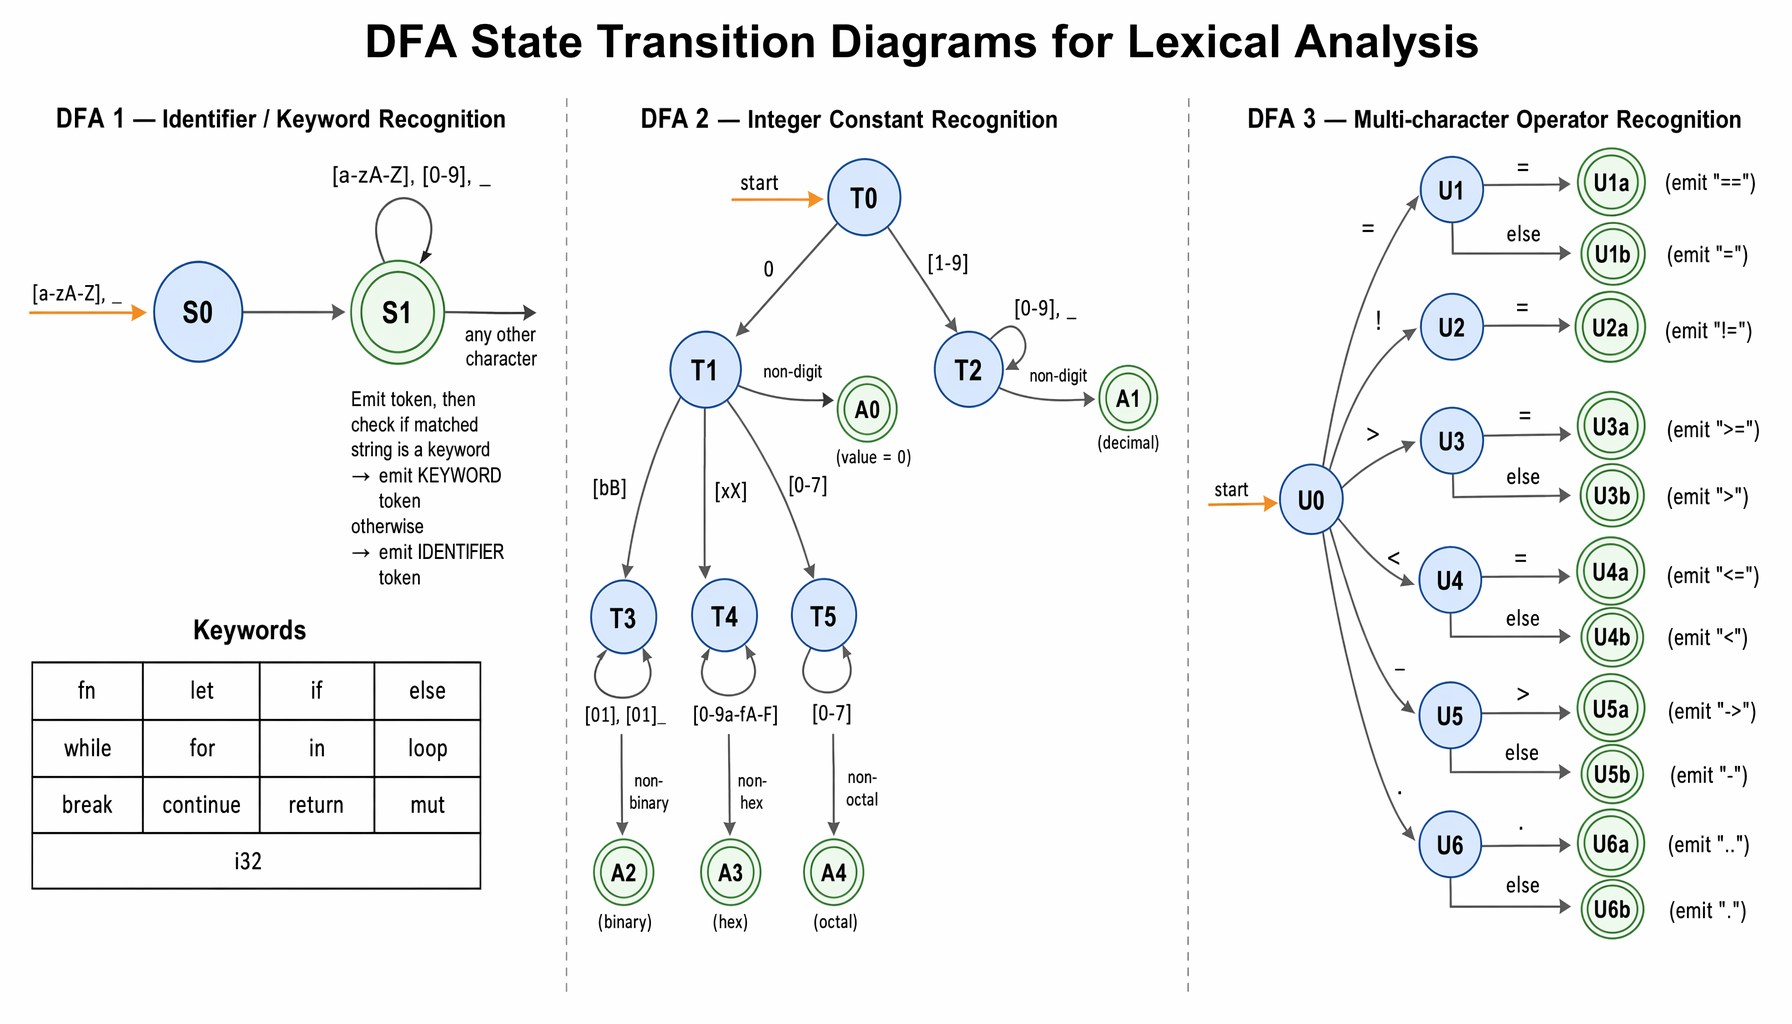
\includegraphics[width=\textwidth]{figures/dfa_state_transition.png}
    \caption{词法分析有限状态自动机示意图}
\end{figure}

Flex工具接受正则表达式作为输入，自动生成对应的有限状态自动机。正则表达式具有以下性质：
\begin{itemize}
    \item 能够表示所有正则语言
    \item 易于书写和理解
    \item 可通过算法转换为等价的DFA
\end{itemize}

\subsection{Flex工具介绍}

Flex是一个快速的词法分析器生成器，是Unix系统中lex工具的免费替代品。其工作流程如下：

\begin{figure}[H]
    \centering
    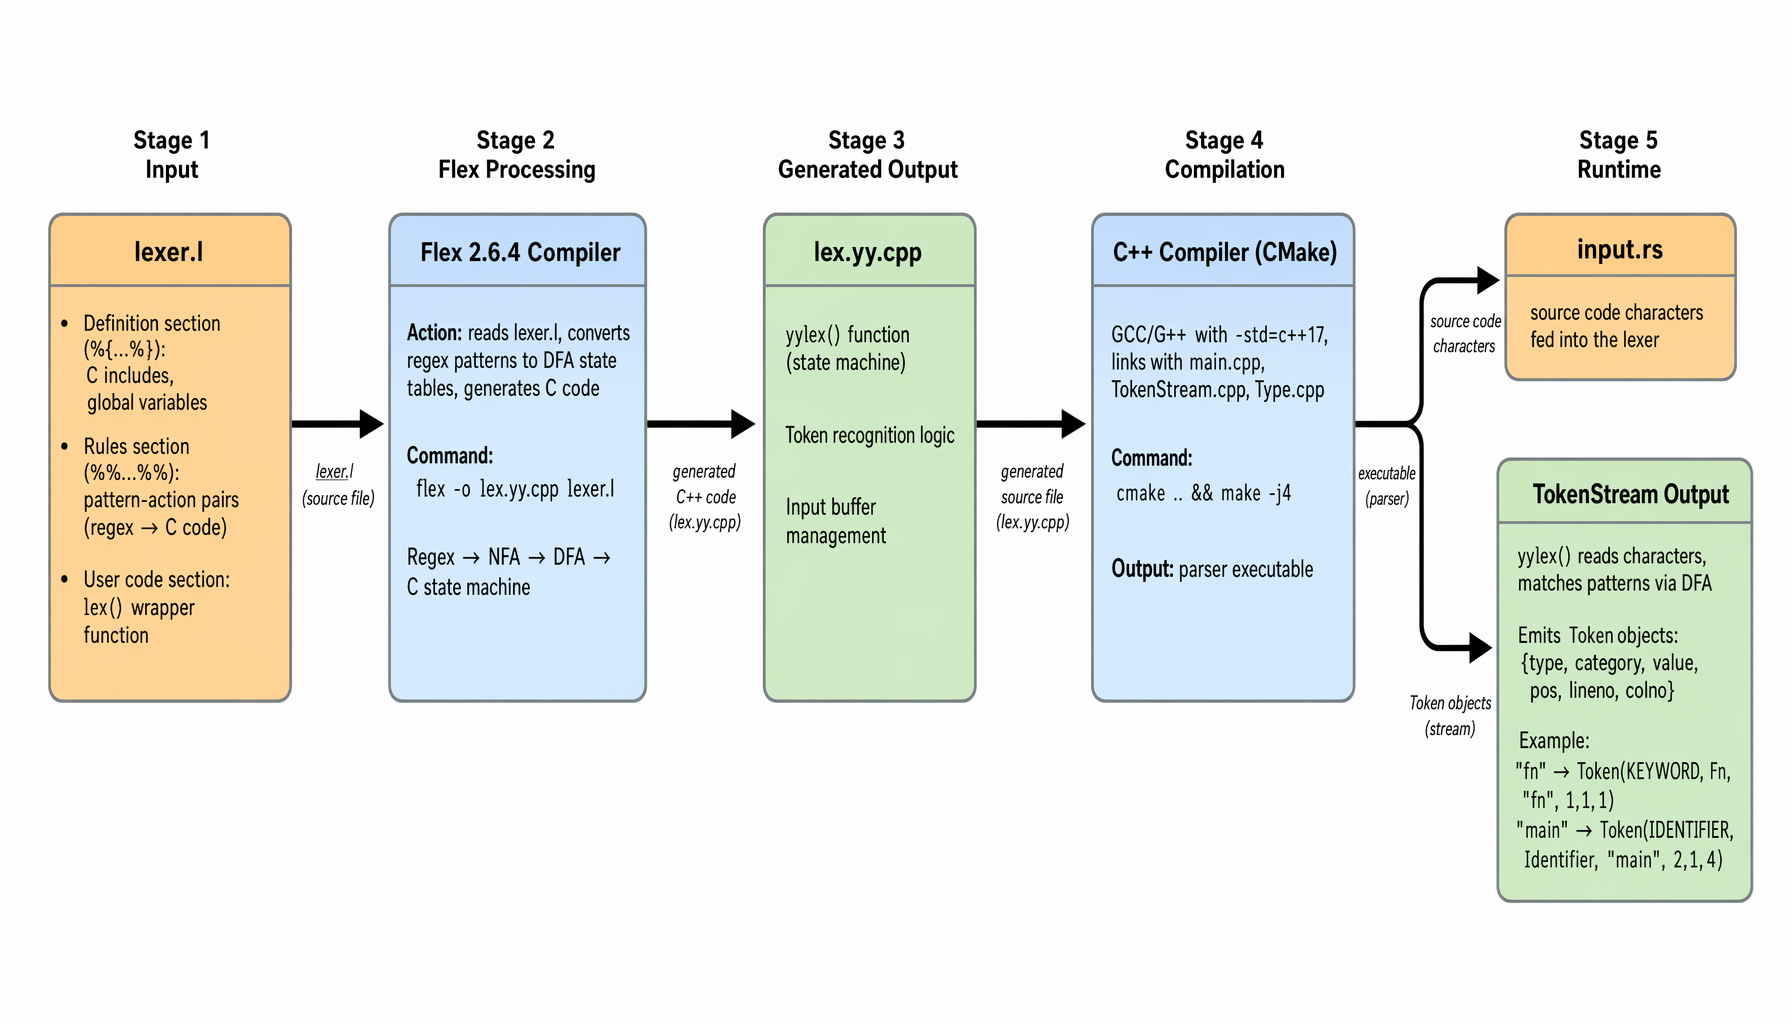
\includegraphics[width=\textwidth]{figures/flex_workflow.png}
    \caption{Flex工作流程图}
\end{figure}

\begin{enumerate}
    \item 编写Flex规则文件（\texttt{.l}），定义正则表达式和对应的动作
    \item Flex读取规则文件，生成C语言源文件（\texttt{lex.yy.c}）
    \item 编译生成的C文件，得到词法分析器可执行程序
    \item 运行词法分析器，输入源代码，输出Token序列
\end{enumerate}

Flex规则文件的基本结构：

\begin{lstlisting}[language=C, caption={Flex规则文件结构}]
%{
/* C代码声明区：头文件、全局变量、辅助函数 */
#include "TokenStream.h"
#include "Token.h"
%}

/* Flex选项定义 */
%option yylineno
%option noyywrap

/* 正则表达式宏定义 */
DIGIT    [0-9]
LETTER   [a-zA-Z]
...

%%
/* 规则区：正则表达式 + 动作 */
{LETTER}({LETTER}|{DIGIT})*   { /* 标识符动作 */ }
...

%%
/* 用户代码区：辅助函数实现 */
\end{lstlisting}

\subsection{Token设计}

Token是词法分析的基本输出单位，包含类型、种别、值、位置等信息。

\subsubsection{Type枚举定义}

\begin{lstlisting}[language=C++, caption={Type枚举定义（Type.h）}]
enum class Type {
    KEYWORD,      // 关键字
    OPERATOR,     // 运算符
    DELIMITER,    // 界符
    CONSTANT,     // 常量
    IDENTIFIER,   // 标识符
    DECLERATOR,   // 类型声明符
    COMMENT,      // 注释
    TYPE_EOF      // 文件结束
};
\end{lstlisting}

\subsubsection{Token类定义}

\begin{lstlisting}[language=C++, caption={Token类定义（Token.h）}]
class Token {
public:
    Type type;         // Token类型
    string category;   // 种别码
    string value;      // 原始文本值
    int pos;           // 在Token流中的位置
    int lineno;        // 行号（用于错误报告）
    int colno;         // 列号（用于错误报告）

    Token() = default;
    Token(Type t, const string& cat, const string& val,
          int p = 0, int ln = 0, int cn = 0)
        : type(t), category(cat), value(val),
          pos(p), lineno(ln), colno(cn) {}
};
\end{lstlisting}

Token设计考虑了以下因素：
\begin{itemize}
    \item \textbf{类型区分}：通过Type枚举快速判断Token大类
    \item \textbf{种别码细化}：通过category区分同类型的不同Token
    \item \textbf{位置信息}：记录行列号，便于语法分析时报错定位
\end{itemize}

\subsection{正则表达式规则设计}

\subsubsection{常量识别规则}

常量识别是词法分析中最复杂的部分，需要支持多种进制和格式。

\begin{lstlisting}[language=Flex, basicstyle=\ttfamily\scriptsize, caption={常量正则表达式规则}]
/* 数字基础定义 */
DIGIT                    [0-9]
NoneZeroDigit            [1-9]
OctalDigit               [0-7]
HexadecimalDigit         [0-9a-fA-F]
BinaryDigit              [01]

/* 整数后缀 */
IntegerSuffix            (i8|i16|i32|i64|i128|u8|u16|u32|u64|u128|isize|usize)

/* 各种进制整数 */
BinaryConstant           0[bB]({BinaryDigit}+|{BinaryDigit}({BinaryDigit}_)*{BinaryDigit})
OctalConstant            0{OctalDigit}+
HexadecimalConstant      0[xX]({HexadecimalDigit}+|{HexadecimalDigit}({HexadecimalDigit}_)*{HexadecimalDigit})
DecimalConstant          ({NoneZeroDigit}{DIGIT}*|{NoneZeroDigit}({DIGIT}|_)*{DIGIT}|0)

/* 整数常量（合并） */
IntegerConstant          ({DecimalConstant}{IntegerSuffix}?|{HexadecimalConstant}{IntegerSuffix}?|{BinaryConstant})

/* 浮点常量 */
FractionalConstant       ({DigitSequence}?\.{DigitSequence}|{DigitSequence}\.)
ExponentPart             [eE][+-]?{DigitSequence}
FloatingSuffix           [fFlL]
FloatingConstant         {FractionalConstant}{ExponentPart}?{FloatingSuffix}?

/* 字符串常量 */
SChar                    ([^"\\\r\n]|{EscapeSequence}|\\\n|\\\r\n)
StringConst              \"{SChar}*\"

/* 字符常量 */
CChar                    [^'\\\r\n]|{EscapeSequence}
CharacterConstant        \'{CChar}+\'
\end{lstlisting}

\subsubsection{关键字识别规则}

关键字需要优先于标识符识别，以避免误判。

\begin{lstlisting}[language=Flex, caption={关键字识别规则}]
/* 关键字必须放在标识符规则之前 */
let      { CURRENT_TOKEN = Token(Type::KEYWORD, "Let", yytext, ...); return 1; }
mut      { CURRENT_TOKEN = Token(Type::KEYWORD, "Mut", yytext, ...); return 1; }
fn       { CURRENT_TOKEN = Token(Type::KEYWORD, "Fn", yytext, ...); return 1; }
if       { CURRENT_TOKEN = Token(Type::KEYWORD, "If", yytext, ...); return 1; }
else     { CURRENT_TOKEN = Token(Type::KEYWORD, "Else", yytext, ...); return 1; }
while    { CURRENT_TOKEN = Token(Type::KEYWORD, "While", yytext, ...); return 1; }
for      { CURRENT_TOKEN = Token(Type::KEYWORD, "For", yytext, ...); return 1; }
in       { CURRENT_TOKEN = Token(Type::KEYWORD, "In", yytext, ...); return 1; }
loop     { CURRENT_TOKEN = Token(Type::KEYWORD, "Loop", yytext, ...); return 1; }
break    { CURRENT_TOKEN = Token(Type::KEYWORD, "Break", yytext, ...); return 1; }
continue { CURRENT_TOKEN = Token(Type::KEYWORD, "Continue", yytext, ...); return 1; }
return   { CURRENT_TOKEN = Token(Type::KEYWORD, "Return", yytext, ...); return 1; }

/* 类型声明符 */
i32      { CURRENT_TOKEN = Token(Type::DECLERATOR, "I32", yytext, ...); return 1; }
\end{lstlisting}

\subsubsection{关键字与标识符的区分机制}

作业明确要求验证以下边界情况：

\begin{lstlisting}[language=RustLike]
if123       // 应识别为标识符
if=123      // 应识别为三个 Token: (if, 关键字) (=, 算符) (123, 整数)
\end{lstlisting}

Flex 采用\textbf{最长匹配}（Maximal Munch）原则：在所有能匹配当前输入的正则表达式中，选择匹配\textbf{最长字符串}的那条规则；若长度相同，则选择在规则文件中\textbf{先出现}的那条。

对于 \texttt{if123}：
\begin{itemize}
    \item 关键字规则 \texttt{if} 匹配 2 个字符
    \item 标识符规则 $\{Identifier\}$ 匹配 5 个字符（\texttt{if123} 整体符合"字母开头、后跟字母数字下划线"的模式）
    \item 最长匹配原则选择标识符规则，\texttt{if123} 被正确识别为标识符
\end{itemize}

对于 \texttt{if=123}：
\begin{itemize}
    \item 首次匹配时，关键字 \texttt{if} 和标识符前缀 \texttt{i} 均可匹配，但 \texttt{if} 之后的 \texttt{=} 不是字母/数字/下划线，因此标识符规则最多匹配 2 个字符（\texttt{if}），与关键字规则长度相同
    \item 长度相同时，Flex 选择先出现的规则——关键字 \texttt{if} 的规则位于标识符规则之前，因此 \texttt{if} 被识别为关键字
    \item 随后 \texttt{=} 匹配赋值号界符，\texttt{123} 匹配整数常量
    \item 最终产生三个 Token：\texttt{(keyword, If, if)}、\texttt{(delimiter, Assign, =)}、\texttt{(constant, IntegerConstant, 123)}
\end{itemize}

这种机制保证了关键字不会被误识别为标识符前缀，同时也允许以关键字为前缀的合法标识符（如 \texttt{if123}、\texttt{let\_x}）被正确识别。

\subsubsection{运算符与界符识别}

\begin{lstlisting}[language=Flex, caption={运算符与界符识别规则}]
/* 运算符（注意顺序：长运算符优先） */
"->"     { CURRENT_TOKEN = Token(Type::OPERATOR, "Arrow", yytext, ...); return 1; }
".."     { CURRENT_TOKEN = Token(Type::OPERATOR, "DotDot", yytext, ...); return 1; }
"."      { CURRENT_TOKEN = Token(Type::OPERATOR, "Dot", yytext, ...); return 1; }
"=="     { CURRENT_TOKEN = Token(Type::OPERATOR, "EqualEqual", yytext, ...); return 1; }
"!="     { CURRENT_TOKEN = Token(Type::OPERATOR, "NotEqual", yytext, ...); return 1; }
">="     { CURRENT_TOKEN = Token(Type::OPERATOR, "GreaterEqual", yytext, ...); return 1; }
"<="     { CURRENT_TOKEN = Token(Type::OPERATOR, "LessEqual", yytext, ...); return 1; }
">"      { CURRENT_TOKEN = Token(Type::OPERATOR, "Greater", yytext, ...); return 1; }
"<"      { CURRENT_TOKEN = Token(Type::OPERATOR, "Less", yytext, ...); return 1; }
"+"      { CURRENT_TOKEN = Token(Type::OPERATOR, "Plus", yytext, ...); return 1; }
"-"      { CURRENT_TOKEN = Token(Type::OPERATOR, "Minus", yytext, ...); return 1; }
"*"      { CURRENT_TOKEN = Token(Type::OPERATOR, "Star", yytext, ...); return 1; }
"/"      { CURRENT_TOKEN = Token(Type::OPERATOR, "Slash", yytext, ...); return 1; }
"&"      { CURRENT_TOKEN = Token(Type::OPERATOR, "Ampersand", yytext, ...); return 1; }

/* 界符 */
"="      { CURRENT_TOKEN = Token(Type::DELIMITER, "Assign", yytext, ...); return 1; }
";"      { CURRENT_TOKEN = Token(Type::DELIMITER, "Semicolon", yytext, ...); return 1; }
":"      { CURRENT_TOKEN = Token(Type::DELIMITER, "Colon", yytext, ...); return 1; }
","      { CURRENT_TOKEN = Token(Type::DELIMITER, "Comma", yytext, ...); return 1; }
"("      { CURRENT_TOKEN = Token(Type::DELIMITER, "LParen", yytext, ...); return 1; }
")"      { CURRENT_TOKEN = Token(Type::DELIMITER, "RParen", yytext, ...); return 1; }
"{"      { CURRENT_TOKEN = Token(Type::DELIMITER, "LBrace", yytext, ...); return 1; }
"}"      { CURRENT_TOKEN = Token(Type::DELIMITER, "RBrace", yytext, ...); return 1; }
"["      { CURRENT_TOKEN = Token(Type::DELIMITER, "LBracket", yytext, ...); return 1; }
"]"      { CURRENT_TOKEN = Token(Type::DELIMITER, "RBracket", yytext, ...); return 1; }
\end{lstlisting}

\subsection{输出格式设计}

词法分析器输出采用TSV（Tab-Separated Values）格式，便于后续处理和可视化。

\begin{table}[H]
\centering
\caption{词法分析输出格式示例}
\begin{tabular}{|l|l|l|}
\hline
\textbf{Type} & \textbf{Category} & \textbf{Value} \\
\hline
keyword & Let & let \\
keyword & Mut & mut \\
identifier & Identifier & x \\
delimiter & Assign & = \\
constant & IntegerConstant & 42 \\
delimiter & Semicolon & ; \\
\hline
\end{tabular}
\end{table}

输出格式设计说明：
\begin{itemize}
    \item \textbf{首行表头}：标注各列含义
    \item \textbf{分隔符}：使用制表符（\texttt{\textbackslash t}），便于程序解析
    \item \textbf{注释过滤}：语法分析时自动跳过注释Token
    \item \textbf{特殊字符转义}：对于字符串中的换行等特殊字符，采用自定义转义规则
\end{itemize}

\subsection{TokenStream接口}

TokenStream类作为词法分析器与语法分析器之间的桥梁，提供流式Token访问接口。

\begin{lstlisting}[language=C++, caption={TokenStream核心接口}]
class TokenStream {
protected:
    vector<Token> toks;  // Token存储
    int cur = 0;         // 当前位置指针

public:
    void load(istream& in);            // 加载Token流
    const Token& peek(int offset = 0); // 查看当前Token（不移动指针）
    Token advance();                   // 获取当前Token并移动指针
    Token expect(const string& cat);   // 期望特定种别，否则报错
    bool check(const string& cat);     // 检查当前Token是否匹配
    bool atEnd();                      // 判断是否到达末尾
};
\end{lstlisting}

\begin{figure}[H]
    \centering
    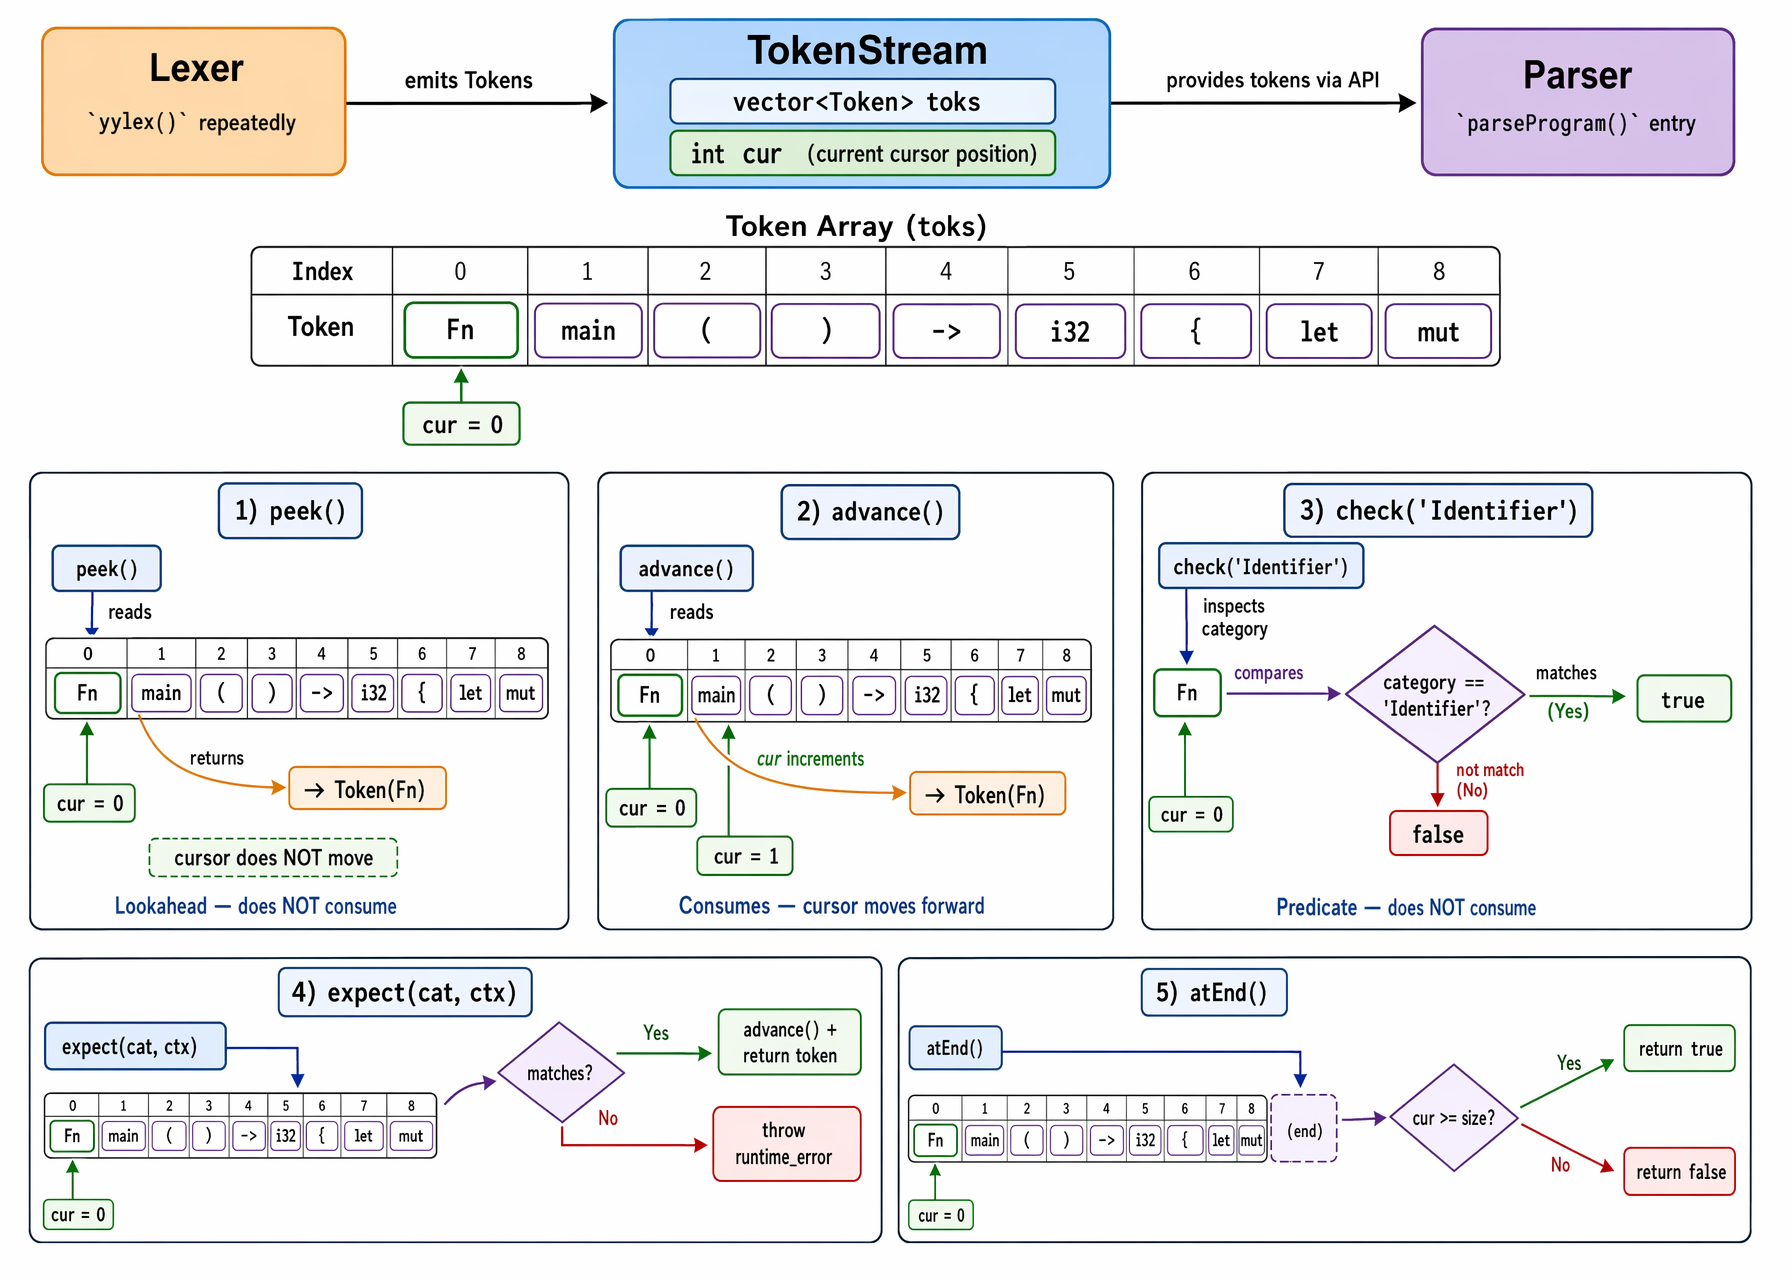
\includegraphics[width=\textwidth]{figures/tokenstream_mechanism.png}
    \caption{TokenStream工作原理图}
\end{figure}

\newpage

% ============================================================
%  第四章 语法分析器设计与实现
% ============================================================
\section{语法分析器设计与实现}

语法分析是编译过程的第二阶段，负责将Token序列组织成语法树。本章详细介绍递归下降语法分析器的设计与实现。

\subsection{语法分析理论基础}

\subsubsection{递归下降分析法原理}

递归下降分析法（Recursive Descent Parsing）是一种自顶向下的语法分析方法，其核心思想是：
\begin{itemize}
    \item 为每个非终结符编写一个对应的递归函数
    \item 函数根据当前Token选择匹配的产生式
    \item 通过递归调用处理嵌套结构
\end{itemize}

\begin{figure}[H]
    \centering
    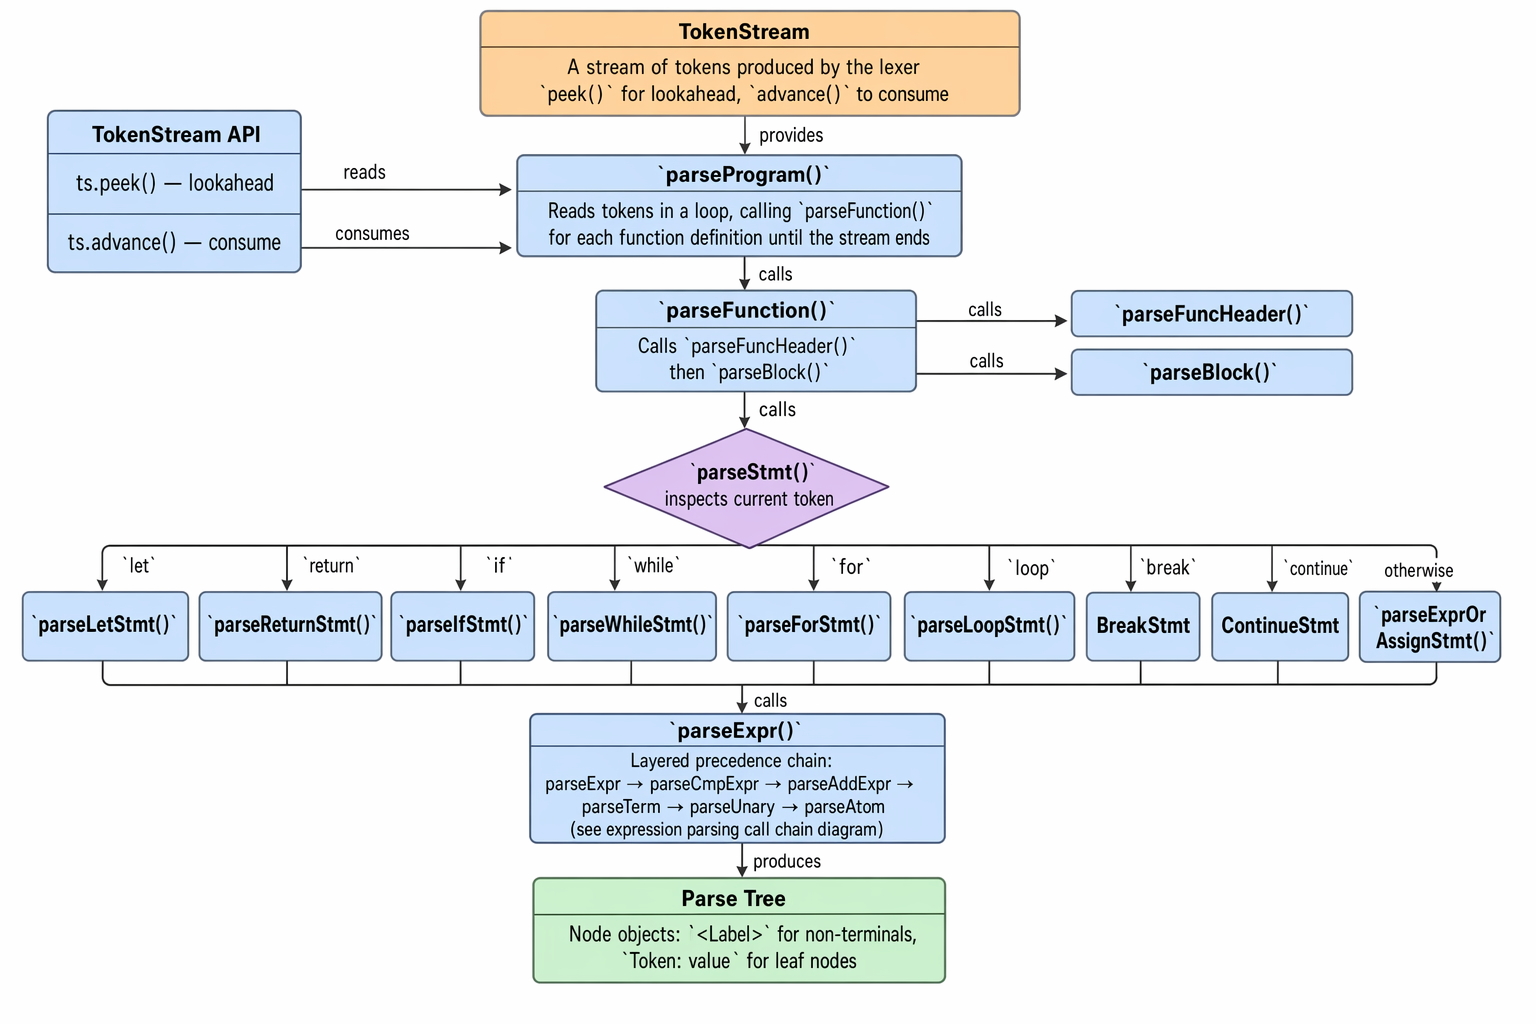
\includegraphics[width=\textwidth]{figures/recursive_descent_flow.png}
    \caption{递归下降分析流程图}
\end{figure}

递归下降分析的特点：
\begin{enumerate}
    \item \textbf{优点}：
        \begin{itemize}
            \item 实现简单直观，易于理解和调试
            \item 可以灵活添加错误处理和恢复机制
            \item 便于扩展和修改文法规则
        \end{itemize}
    \item \textbf{局限性}：
        \begin{itemize}
            \item 要求文法满足LL(1)条件
            \item 需要消除左递归
            \item 对某些复杂文法处理困难
        \end{itemize}
\end{enumerate}

\subsubsection{LL(1)文法判定}

LL(1)文法是指可以从左向右扫描输入、进行最左推导、仅使用1个向前查看符号的文法。判断文法是否为LL(1)需满足：
\begin{enumerate}
    \item 无左递归
    \item 无公共左因子
    \item 对于每个非终结符A的两个产生式 $A \rightarrow \alpha | \beta$，满足 $FIRST(\alpha) \cap FIRST(\beta) = \emptyset$
\end{enumerate}

\subsubsection{左递归消除方法}

左递归是指形如 $A \rightarrow A\alpha | \beta$ 的产生式。直接左递归可通过以下公式消除：

设 $A \rightarrow A\alpha_1 | A\alpha_2 | ... | A\alpha_n | \beta_1 | \beta_2 | ... | \beta_m$

转换为：
\begin{align}
A &\rightarrow \beta_1 A' | \beta_2 A' | ... | \beta_m A' \\
A' &\rightarrow \alpha_1 A' | \alpha_2 A' | ... | \alpha_n A' | \epsilon
\end{align}

例如，表达式文法 $E \rightarrow E + T | T$ 消除左递归后：
\begin{align}
E &\rightarrow T E' \\
E' &\rightarrow + T E' | \epsilon
\end{align}

\subsection{语法树数据结构}

语法树（Parse Tree）是语法分析的输出结果，反映了源代码的语法结构。

\subsubsection{Node类定义}

\begin{lstlisting}[language=C++, caption={Node类定义}]
class Node {
public:
    string label;                  // 节点标签（如"IfStmt", "Identifier"）
    vector<unique_ptr<Node>> children; // 子节点列表
    bool isLeaf = false;           // 是否为叶节点

    explicit Node(string lbl, bool leaf = false)
        : label(move(lbl)), isLeaf(leaf) {}

    void PrintToFile(ofstream& ofs, int depth = 0) const;
};
\end{lstlisting}

\subsubsection{辅助函数}

\begin{lstlisting}[language=C++, caption={语法树辅助函数}]
using NodePtr = unique_ptr<Node>;

// 创建非叶节点
static inline NodePtr makeNode(const string& lbl) {
    return make_unique<Node>(lbl);
}

// 创建叶节点（Token）
static inline NodePtr makeLeaf(const string& lbl) {
    return make_unique<Node>(lbl, true);
}

// 添加子节点
static inline void addChild(NodePtr& parent, NodePtr child) {
    parent->children.push_back(move(child));
}
\end{lstlisting}

\begin{figure}[H]
    \centering
    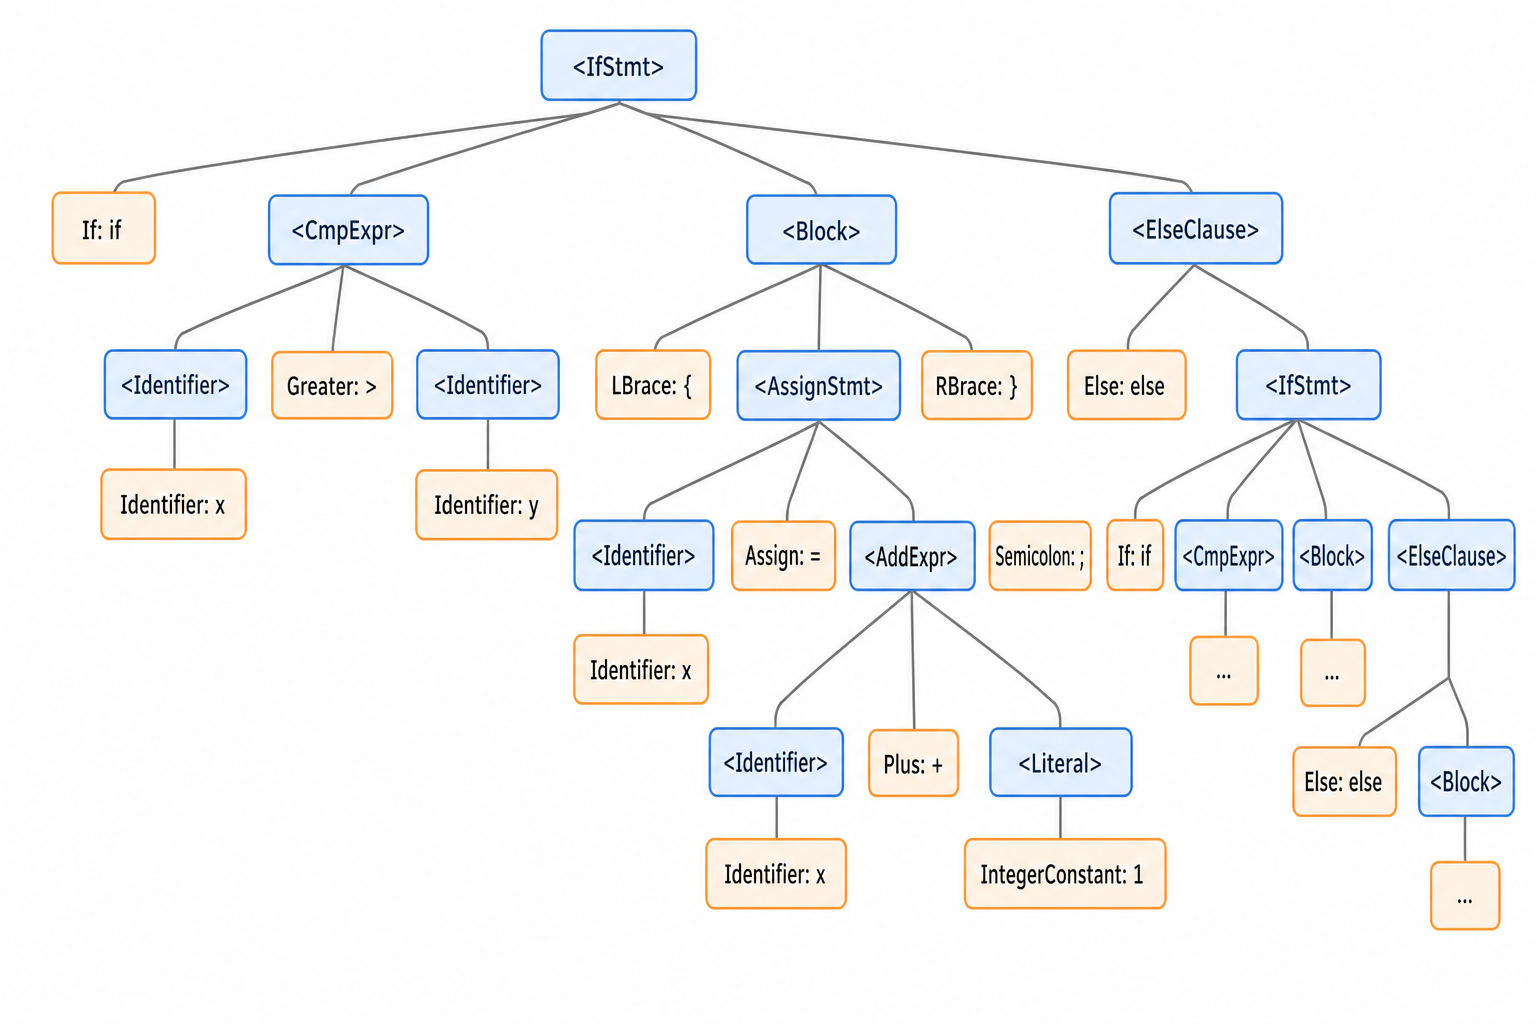
\includegraphics[width=\textwidth]{figures/parse_tree_structure.png}
    \caption{语法树结构示意图（if-else 语句）}
\end{figure}

\subsection{Parser类实现}

Parser类是语法分析器的核心，封装了所有解析函数。

\begin{lstlisting}[language=C++, caption={Parser类框架}]
class Parser {
    TokenStream& ts;  // Token流引用

    // 辅助函数
    NodePtr consumeLeaf();                    // 消耗Token，生成叶节点
    NodePtr expectLeaf(const string& cat);    // 期望特定Token

public:
    explicit Parser(TokenStream& ts) : ts(ts) {}

    NodePtr parse();          // 入口：解析整个程序
    NodePtr parseProgram();   // 解析程序
    NodePtr parseFunction();  // 解析函数
    NodePtr parseStmt();      // 解析语句（分发）
    NodePtr parseExpr();      // 解析表达式
    // ... 其他解析函数
};
\end{lstlisting}

\subsubsection{核心解析函数示例}

\textbf{if语句解析函数}：

\begin{lstlisting}[language=C++, caption={parseIfStmt函数实现}]
NodePtr parseIfStmt() {
    auto node = makeNode("IfStmt");
    addChild(node, expectLeaf("If"));      // if关键字
    addChild(node, parseExpr());           // 条件表达式
    addChild(node, parseBlock());          // if块

    if (ts.check("Else")) {
        auto elseNode = makeNode("ElseClause");
        addChild(elseNode, consumeLeaf()); // else关键字
        if (ts.check("If")) {
            addChild(elseNode, parseIfStmt()); // else-if
        } else {
            addChild(elseNode, parseBlock());  // else块
        }
        addChild(node, move(elseNode));
    }
    return node;
}
\end{lstlisting}

\textbf{let语句解析函数}：

\begin{lstlisting}[language=C++, caption={parseLetStmt函数实现}]
NodePtr parseLetStmt() {
    auto node = makeNode("LetStmt");
    addChild(node, expectLeaf("Let"));

    // 变量声明
    auto decl = makeNode("VarDecl");
    if (ts.check("Mut")) addChild(decl, consumeLeaf()); // [mut]
    addChild(decl, expectLeaf("Identifier", "variable name"));
    if (ts.check("Colon")) {
        addChild(decl, consumeLeaf());
        addChild(decl, parseType());  // [: Type]
    }
    addChild(node, move(decl));

    // 初始化表达式
    if (ts.check("Assign")) {
        addChild(node, consumeLeaf());
        addChild(node, parseExpr());  // [= Expr]
    }
    addChild(node, expectLeaf("Semicolon"));
    return node;
}
\end{lstlisting}

\textbf{语句分发函数}：

\begin{lstlisting}[language=C++, caption={parseStmt语句分发}]
NodePtr parseStmt() {
    const Token& tok = ts.peek();

    if (tok.category == "Semicolon") return parseEmptyStmt();
    if (tok.category == "Let")       return parseLetStmt();
    if (tok.category == "Return")    return parseReturnStmt();
    if (tok.category == "If")        return parseIfStmt();
    if (tok.category == "While")     return parseWhileStmt();
    if (tok.category == "For")       return parseForStmt();
    if (tok.category == "Loop")      return parseLoopStmt();
    if (tok.category == "Break")     return parseBreakStmt();
    if (tok.category == "Continue")  return parseContinueStmt();
    if (tok.category == "LBrace")    return parseBlock();

    // 其他：赋值语句或表达式语句
    return parseExprOrAssignStmt();
}
\end{lstlisting}

\subsection{表达式解析与运算符优先级}

表达式解析需要正确处理运算符优先级。本项目采用分层递归的方法，每层对应一个优先级。

\begin{table}[H]
\centering
\caption{运算符优先级层次}
\begin{tabular}{|c|l|l|l|}
\hline
\textbf{层次} & \textbf{函数名} & \textbf{运算符} & \textbf{优先级} \\
\hline
1 & parseExpr & \texttt{..}（范围） & 最低 \\
\hline
2 & parseCmpExpr & \texttt{== != > >= < <=} & 低 \\
\hline
3 & parseAddExpr & \texttt{+ -} & 中低 \\
\hline
4 & parseTerm & \texttt{* /} & 中高 \\
\hline
5 & parseUnary & \texttt{\& * \&mut}（单目） & 高 \\
\hline
6 & parseAtom & 常量、标识符等 & 最高 \\
\hline
\end{tabular}
\end{table}

\subsubsection{表达式解析函数}

\begin{lstlisting}[language=C++, caption={表达式解析函数系列}]
// Expr -> CmpExpr ['..' CmpExpr]
NodePtr parseExpr() {
    NodePtr lhs = parseCmpExpr();
    if (ts.check("DotDot")) {
        auto node = makeNode("RangeExpr");
        addChild(node, move(lhs));
        addChild(node, consumeLeaf());
        addChild(node, parseCmpExpr());
        return node;
    }
    return lhs;
}

// CmpExpr -> AddExpr { CmpOp AddExpr }
NodePtr parseCmpExpr() {
    NodePtr lhs = parseAddExpr();
    while (isCmpOp()) {  // == != > >= < <=
        auto node = makeNode("CmpExpr");
        addChild(node, move(lhs));
        addChild(node, consumeLeaf());
        addChild(node, parseAddExpr());
        lhs = move(node);
    }
    return lhs;
}

// AddExpr -> Term { ('+'|'-') Term }
NodePtr parseAddExpr() {
    NodePtr lhs = parseTerm();
    while (ts.check("Plus") || ts.check("Minus")) {
        auto node = makeNode("AddExpr");
        addChild(node, move(lhs));
        addChild(node, consumeLeaf());
        addChild(node, parseTerm());
        lhs = move(node);
    }
    return lhs;
}

// Term -> Unary { ('*'|'/') Unary }
NodePtr parseTerm() {
    NodePtr lhs = parseUnary();
    while (ts.check("Star") || ts.check("Slash")) {
        auto node = makeNode("MulExpr");
        addChild(node, move(lhs));
        addChild(node, consumeLeaf());
        addChild(node, parseUnary());
        lhs = move(node);
    }
    return lhs;
}

// Unary -> '&' ['mut'] Unary | '*' Unary | Atom
NodePtr parseUnary() {
    if (ts.check("Ampersand")) {
        auto node = makeNode("RefExpr");
        addChild(node, consumeLeaf());
        if (ts.check("Mut")) addChild(node, consumeLeaf());
        addChild(node, parseUnary());
        return node;
    }
    if (ts.check("Star")) {
        auto node = makeNode("DerefExpr");
        addChild(node, consumeLeaf());
        addChild(node, parseUnary());
        return node;
    }
    return parseAtom();
}
\end{lstlisting}

\begin{figure}[H]
    \centering
    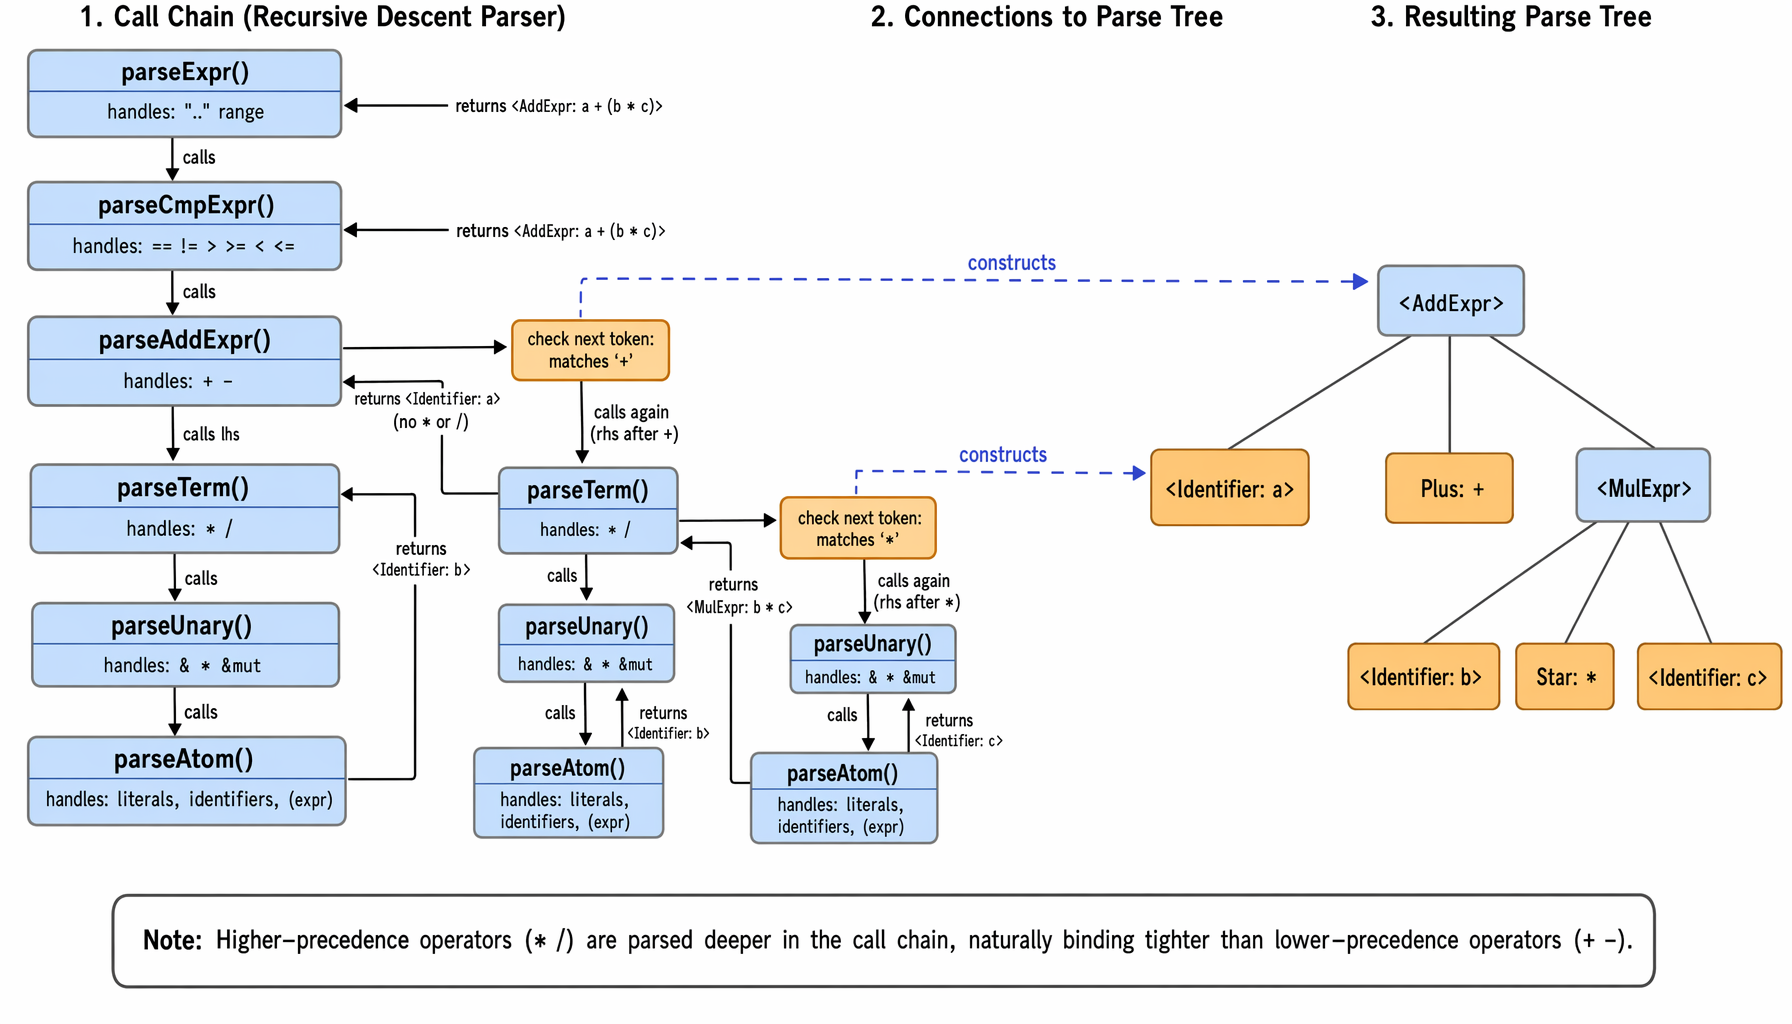
\includegraphics[width=\textwidth]{figures/expression_call_chain.png}
    \caption{表达式解析调用链图}
\end{figure}

\newpage

% ============================================================
%  第五章 GUI可视化模块
% ============================================================
\section{GUI可视化模块}

为了提供直观的分析结果展示，本项目基于ImGui框架实现了图形化界面。本章介绍GUI模块的设计与实现。

\subsection{ImGui框架简介}

ImGui（Immediate Mode GUI）是一个轻量级的C++ GUI库，具有以下特点：
\begin{itemize}
    \item \textbf{即时模式}：界面状态在每帧重新计算，无需持久化存储
    \item \textbf{易于集成}：可直接嵌入现有渲染管线
    \item \textbf{跨平台}：支持多种后端（OpenGL、Vulkan、DirectX等）
    \item \textbf{调试友好}：常用于游戏开发调试工具
\end{itemize}

本项目使用：
\begin{itemize}
    \item \texttt{ImGui}核心库
    \item \texttt{GLFW}窗口管理
    \item \texttt{OpenGL3}渲染后端
\end{itemize}

\subsection{界面布局设计}

\begin{figure}[H]
    \centering
    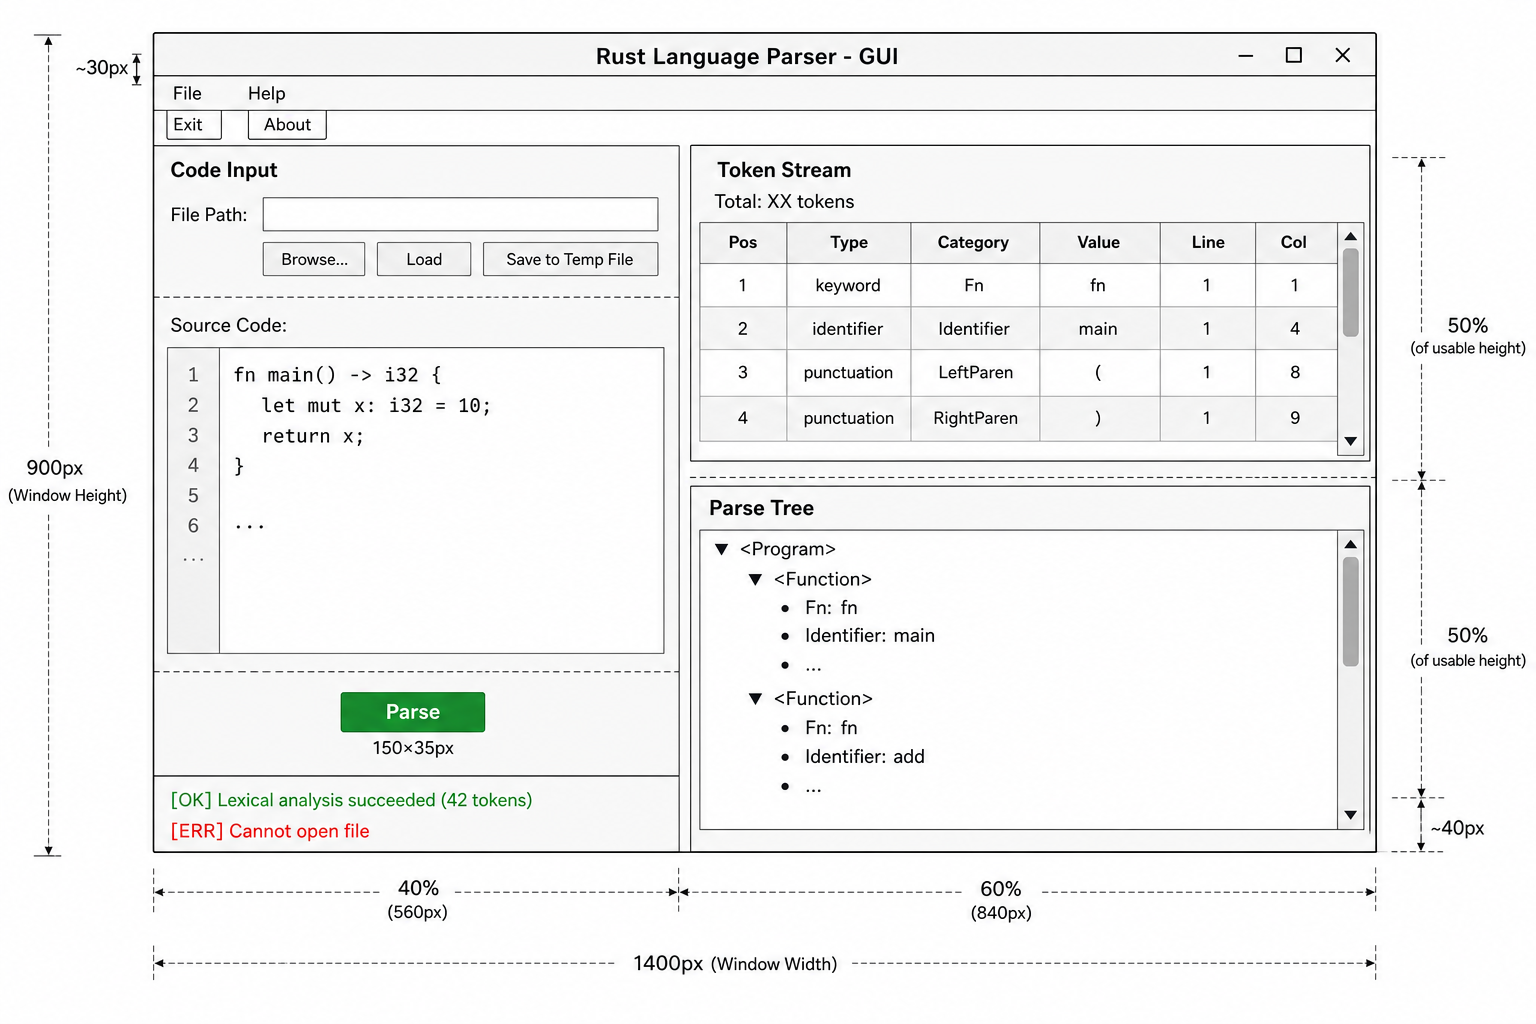
\includegraphics[width=\textwidth]{figures/gui_layout.png}
    \caption{GUI界面布局设计图}
\end{figure}

\subsection{核心组件实现}

\subsubsection{Token列表展示}

\begin{lstlisting}[language=C++, caption={Token列表渲染}]
static void render_token_list() {
    ImGui::Begin("Token Stream");
    ImGui::Text("Total: %zu tokens", g_state.tokens.size());

    if (ImGui::BeginTable("Tokens", 6,
        ImGuiTableFlags_Borders | ImGuiTableFlags_RowBg)) {
        ImGui::TableSetupColumn("Pos");
        ImGui::TableSetupColumn("Type");
        ImGui::TableSetupColumn("Category");
        ImGui::TableSetupColumn("Value");
        ImGui::TableSetupColumn("Line");
        ImGui::TableSetupColumn("Col");
        ImGui::TableHeadersRow();

        for (const auto& tok : g_state.tokens) {
            ImGui::TableNextRow();
            ImGui::TableSetColumnIndex(0);
            ImGui::Text("%d", tok.pos);
            // ... 其他列
        }
        ImGui::EndTable();
    }
    ImGui::End();
}
\end{lstlisting}

\subsubsection{语法树渲染}

\begin{lstlisting}[language=C++, caption={语法树递归渲染}]
static void render_tree_node(const Node& node, const void* node_ptr) {
    if (node.isLeaf) {
        ImGuiTreeNodeFlags flags = ImGuiTreeNodeFlags_Leaf
            | ImGuiTreeNodeFlags_NoTreePushOnOpen
            | ImGuiTreeNodeFlags_Bullet;
        ImGui::TreeNodeEx(node.label.c_str(), flags);
    } else {
        ImGuiTreeNodeFlags flags = ImGuiTreeNodeFlags_OpenOnArrow
            | ImGuiTreeNodeFlags_OpenOnDoubleClick;
        bool node_open = ImGui::TreeNodeEx(node.label.c_str(), flags);
        if (node_open) {
            for (const auto& child : node.children) {
                render_tree_node(*child, child.get());
            }
            ImGui::TreePop();
        }
    }
}
\end{lstlisting}

\subsection{GUI架构}

\begin{figure}[H]
    \centering
    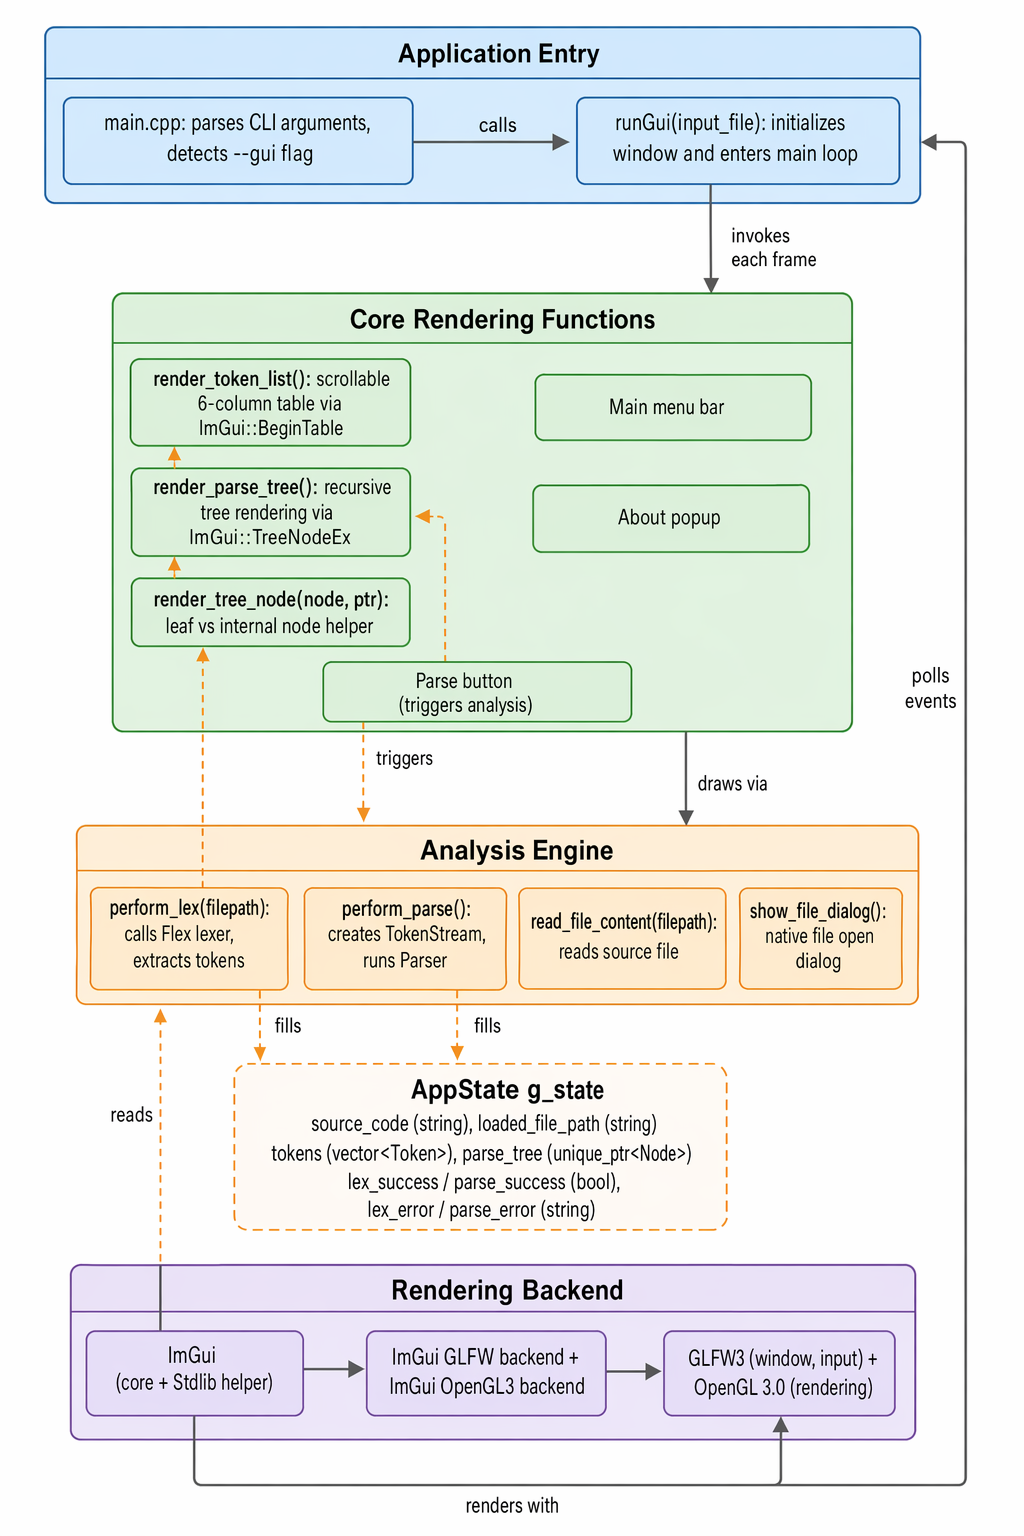
\includegraphics[width=0.9\textwidth]{figures/gui_architecture.png}
    \caption{GUI模块架构图}
\end{figure}

\newpage

% ============================================================
%  第六章 构建与跨平台支持
% ============================================================
\section{构建与跨平台支持}

本项目采用CMake构建系统，支持Linux本地编译和Windows交叉编译。

\subsection{CMake构建系统}

CMake是一个跨平台的构建工具，能够生成各种编译系统的配置文件。

\begin{lstlisting}[language={CMake}, caption={CMakeLists.txt核心配置}]
cmake_minimum_required(VERSION 3.10)
project(Parser VERSION 1.0 LANGUAGES CXX)

# C++17标准
set(CMAKE_CXX_STANDARD 17)
set(CMAKE_CXX_STANDARD_REQUIRED ON)

# 源文件
set(PARSER_SOURCES
    src/main.cpp
    src/TokenStream.cpp
    src/Type.cpp
    src/lex.yy.cpp  # Flex生成
)

# 构建目标
add_executable(parser ${PARSER_SOURCES})
\end{lstlisting}

\subsection{Linux/Windows交叉编译配置}

项目支持在Linux环境下编译Windows可执行文件，使用MinGW-w64工具链。

\begin{figure}[H]
    \centering
    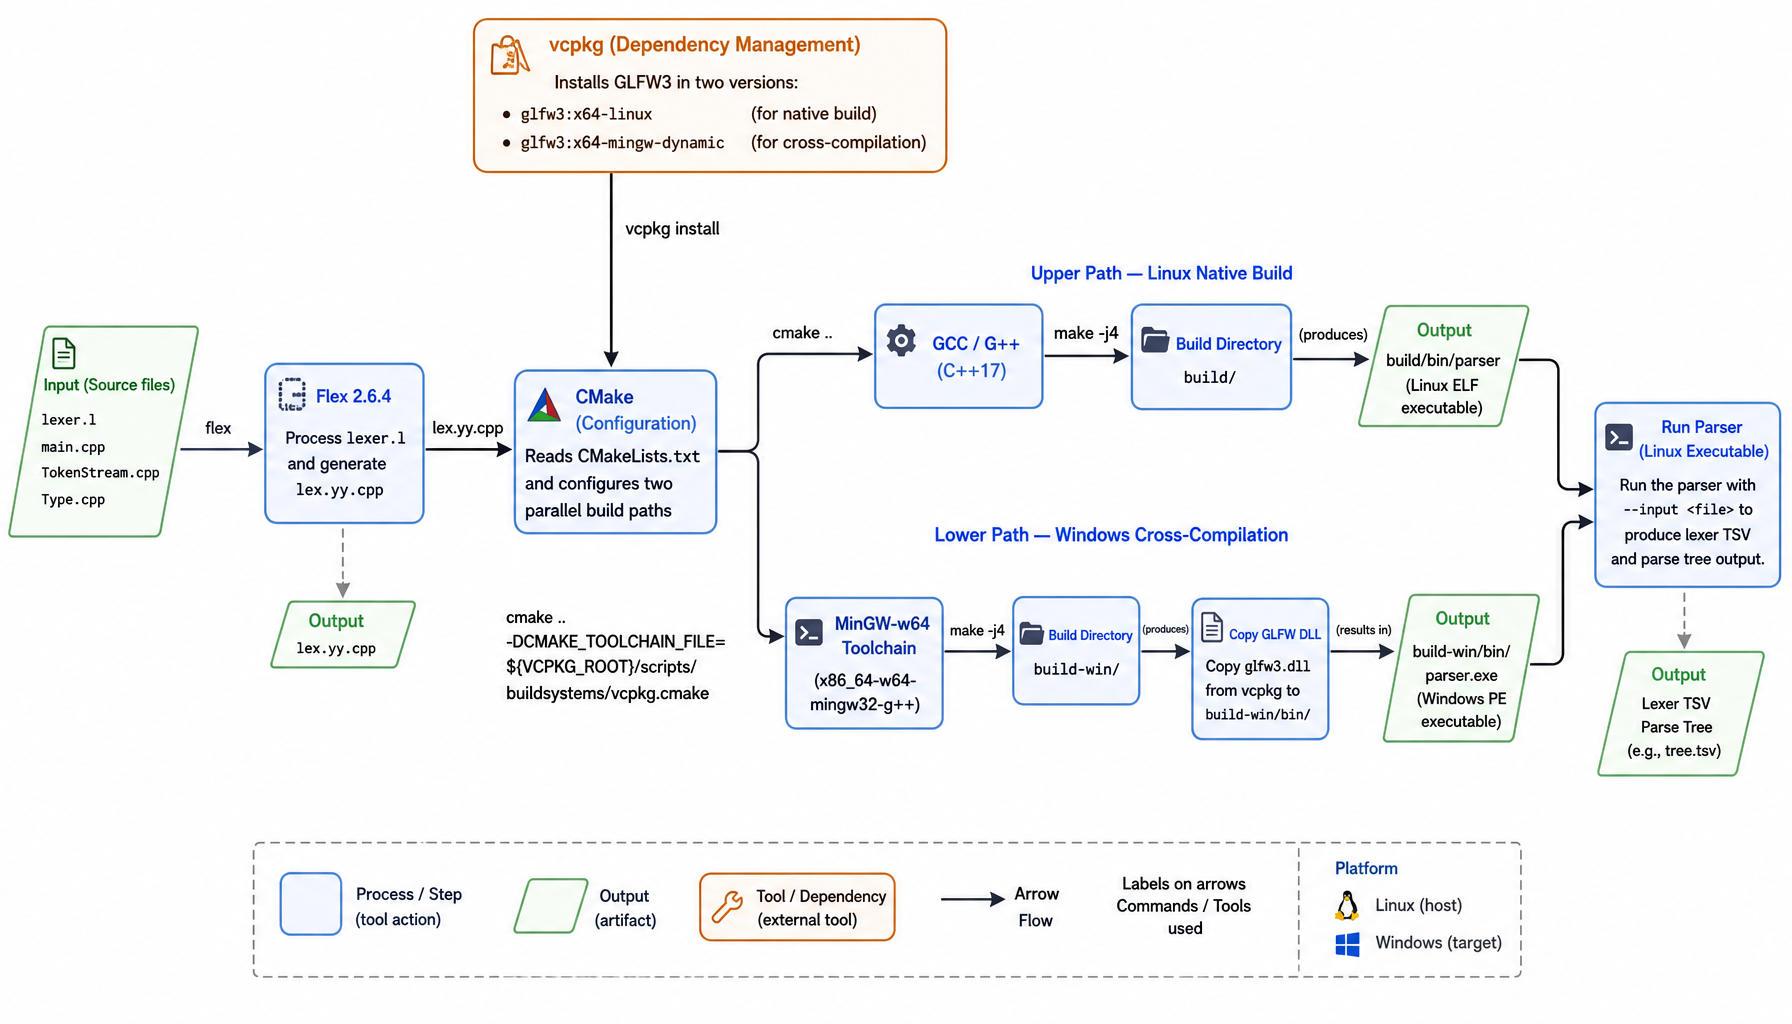
\includegraphics[width=\textwidth]{figures/cross_platform_build.png}
    \caption{跨平台构建流程图}
\end{figure}

\subsection{运行脚本说明}

项目提供\texttt{run.sh}脚本，实现一键构建运行：

\begin{lstlisting}[language=bash, caption={run.sh脚本核心流程}]
#!/bin/bash

# 1. 环境检查与依赖安装
check_dependencies() {
    # 检查flex、g++、cmake、mingw-w64、vcpkg
}

# 2. Flex代码生成
flex -o src/lex.yy.cpp src/lexer.l

# 3. Linux版本编译
mkdir -p build && cd build
cmake ..
make -j4

# 4. Windows版本编译
mkdir -p build-win && cd build-win
cmake .. -DCMAKE_TOOLCHAIN_FILE=/usr/share/cmake/mingw-w64/...
make -j4

# 5. 执行分析
./build/bin/parser --input ./testfiles/input.rs
\end{lstlisting}

\newpage

% ============================================================
%  第七章 测试与结果分析
% ============================================================
\section{测试与结果分析}

本章通过完整的测试用例验证系统的正确性，展示词法分析和语法分析的输出结果。

\subsection{测试用例设计}

测试用例涵盖类Rust语言的主要语法特性：

\begin{lstlisting}[language=RustLike, caption={完整测试输入（input.rs）}]
// this is a single line comment
/* this is a block comment  */

fn main() -> i32 {
    let mut x: i32 = 10;
    let y: i32 = 20;
    let z: i32 = 30;

    // test if-else
    if x > y {
        x = x + 1;
    } else if x < y {
        x = x - 1;
    } else {
        x = 0;
    }

    // test while loop
    while x < 15 {
        x = x + 1;
    }

    // test for-in loop
    for i in 0..10 {
        if i == 5 {
            break;
        }
        continue;
    }

    // test loop loop
    loop {
        x = x + 1;
        if x >= 20 {
            break;
        }
    }

    // test operators
    let a: i32 = x + y;
    let b: i32 = x - y;
    let c: i32 = x * y;
    let d: i32 = x / y;

    // test comparison operators
    let e: bool = x == y;
    let f: bool = x != y;
    let g: bool = x >= y;
    let h: bool = x <= y;

    // test arrays
    let arr: [i32; 3] = [1, 2, 3];
    let val: i32 = arr[0];

    // test function calls
    let result: i32 = add(x, y);

    // test return
    return result;
}

fn add(a: i32, b: i32) -> i32 {
    let sum: i32 = a + b;
    return sum;
}

fn test_special() -> i32 {
    let x: i32 = 100;
    let y: i32 = x;
    let z: i32 = y;

    // test . and ..
    let range = 0..100;

    return x;
}

#
\end{lstlisting}

\subsection{词法分析输出示例}

以下是词法分析器对\texttt{main}函数首部的输出：

\begin{longtable}{|l|l|l|r|}
\caption{词法分析输出示例（main函数首部）} \\
\hline
\textbf{Type} & \textbf{Category} & \textbf{Value} & \textbf{Pos} \\
\hline
\endfirsthead
\hline
\textbf{Type} & \textbf{Category} & \textbf{Value} & \textbf{Pos} \\
\hline
\endhead
\hline
\endfoot
\hline
\endlastfoot

keyword & Fn & fn & 3 \\
identifier & Identifier & main & 4 \\
delimiter & LParen & ( & 5 \\
delimiter & RParen & ) & 6 \\
operator & Arrow & -> & 7 \\
declerator & I32 & i32 & 8 \\
delimiter & LBrace & \{ & 9 \\
keyword & Let & let & 10 \\
keyword & Mut & mut & 11 \\
identifier & Identifier & x & 12 \\
delimiter & Colon & : & 13 \\
declerator & I32 & i32 & 14 \\
delimiter & Assign & = & 15 \\
constant & IntegerConstant & 10 & 16 \\
delimiter & Semicolon & ; & 17 \\
\end{longtable}

\subsection{语法树输出示例}

以下是语法树的部分输出（缩进格式）：

\begin{lstlisting}[language=RustLike, caption={语法树输出示例（IfStmt节点）}]
<IfStmt>
  If: if
  <CmpExpr>
    <Identifier>
      Identifier: x
    Greater: >
    <Identifier>
      Identifier: y
  <Block>
    LBrace: {
    <AssignStmt>
      <Identifier>
        Identifier: x
      Assign: =
      <AddExpr>
        <Identifier>
          Identifier: x
        Plus: +
        <Literal>
          IntegerConstant: 1
      Semicolon: ;
    RBrace: }
  <ElseClause>
    Else: else
    <IfStmt>
      If: if
      <CmpExpr>
        <Identifier>
          Identifier: x
        Less: <
        <Identifier>
          Identifier: y
      <Block>
        ...
\end{lstlisting}

% TODO: 替换为实际截图
% \includegraphics[width=\textwidth]{figures/parse_tree.png}

\subsection{分规则测试用例与结果}

为验证每条文法规则的正确性，我们按规则分组编写了独立的测试文件。测试文件位于 \texttt{parser/testfiles/} 目录下，命名格式为 \texttt{test\_\{规则号\}.rs}。以下展示各组的测试输入及分析结果。

% ----------------------------------------------------------
%  规则 1.1--1.5 程序结构测试
% ----------------------------------------------------------
\subsubsection{程序结构测试（规则 1.1 -- 1.5）}

测试文件 \texttt{test\_1\_1.rs} 至 \texttt{test\_1\_5.rs} 分别对应规则 1.1--1.5：

\begin{lstlisting}[language=RustLike, caption={test\_1\_1.rs -- 空函数（规则 1.1）}]
fn program_1_1() {

}
\end{lstlisting}

\begin{lstlisting}[language=RustLike, caption={test\_1\_2.rs -- 空语句（规则 1.2）}]
fn program_1_2() {
    ;;;;;
}
\end{lstlisting}

\begin{lstlisting}[language=RustLike, caption={test\_1\_3.rs -- 返回语句（规则 1.3）}]
fn program_1_3() {
    return ;
}
\end{lstlisting}

\begin{lstlisting}[language=RustLike, caption={test\_1\_4.rs -- 函数输入：形参列表（规则 1.4）}]
fn program_1_4(mut a:i32) {

}
\end{lstlisting}

\begin{lstlisting}[language=RustLike, caption={test\_1\_5.rs -- 函数输出：返回类型（规则 1.5）}]
fn program_1_5() -> i32 {
    return 1;
}
\end{lstlisting}

测试结果：五个函数均通过语法分析。

% ----------------------------------------------------------
%  规则 2.0--2.3 变量声明与赋值测试
% ----------------------------------------------------------
\subsubsection{变量声明与赋值测试（规则 2.0 -- 2.3）}

测试文件 \texttt{test\_2.rs} 包含三个函数，分别测试规则 2.0--2.3：

\begin{lstlisting}[language=RustLike, caption={test\_2.rs -- 变量声明与赋值（规则 2.0--2.3）}]
fn program_2_1() {
    let mut a;
    let mut b:i32;
}

fn program_2_2(mut a:i32) {
    a=32;
}

fn program_2_3() {
    let mut a=1;
    let mut b:i32=1;
}
\end{lstlisting}

测试结果：三个函数均通过语法分析，语法树正确生成了 \texttt{LetStmt}、\texttt{AssignStmt} 节点。

% ----------------------------------------------------------
%  规则 3.1--3.5 表达式测试
% ----------------------------------------------------------
\subsubsection{表达式测试（规则 3.1 -- 3.5）}

测试文件 \texttt{test\_3.rs} 覆盖了基本表达式、比较运算、加减运算、乘除运算和函数调用：

\begin{lstlisting}[language=RustLike, caption={test\_3.rs -- 表达式（规则 3.1--3.5）}]
fn program_3_1__1() {
    0;
    (1);
    ((2));
    (((3)));
}
fn program_3_1__2(mut a:i32) {
    a;
    (a);
    ((a));
    (((a)));
}
fn program_3_2() {
    1<2;
    3>4;
}
fn program_3_3() {
    1+2;
    3-4;
}
fn program_3_4() {
    1*2;
    3/4;
}

fn program_3_5__1() {

}
fn program_3_5__2() {
    program_3_5__1();
}
\end{lstlisting}

测试结果：全部通过。括号嵌套、比较运算、算术运算和函数调用均被正确解析。

% ----------------------------------------------------------
%  规则 4.1--4.3 选择结构测试
% ----------------------------------------------------------
\subsubsection{选择结构测试（规则 4.1 -- 4.3）}

测试文件 \texttt{test\_4.rs} 覆盖了 if、if-else 和 else if 链：

\begin{lstlisting}[language=RustLike, caption={test\_4.rs -- 选择结构（规则 4.1--4.3）}]
fn program_4_1(a:i32) -> i32 {
    if a>0 {
        return 1;
    }
}
fn program_4_2(a:i32) -> i32 {
    if a>0 {
        return 1;
    } else {
        return 0;
    }
}

fn program_4_3(a:i32) -> i32 {
    if a>0 {
        return a+1;
    } else if a<0 {
        return a-1;
    } else {
        return 0;
    }
}
\end{lstlisting}

测试结果：三个函数均通过。语法分析器正确处理了 \texttt{else if} 的递归嵌套。

% ----------------------------------------------------------
%  规则 5.0--5.4 循环结构测试
% ----------------------------------------------------------
\subsubsection{循环结构测试（规则 5.0 -- 5.4）}

测试文件 \texttt{test\_5.rs} 覆盖了 while、for、loop 和 break/continue：

\begin{lstlisting}[language=RustLike, caption={test\_5.rs -- 循环结构（规则 5.0--5.4）}]
fn program_5_1(mut n:i32) {
    while n>0 {
        n=n-1;
    }
}
fn program_5_2(mut n:i32) {
    for mut i in 1..n+1 {
        n=n-1;
    }
}

fn program_5_3() {
    loop {

    }
}
fn program_5_4() {
    while 1==0 { continue; }
    while 1==1 { break; }
}
\end{lstlisting}

测试结果：四个函数均通过。for 循环的范围表达式 \texttt{1..n+1} 被正确解析为 \texttt{RangeExpr} 节点。

% ----------------------------------------------------------
%  规则 6.1--6.4 引用与借用测试
% ----------------------------------------------------------
\subsubsection{引用与借用测试（规则 6.1 -- 6.4）}

测试文件 \texttt{test\_6.rs} 覆盖了不可变变量、不可变引用、可变引用和解引用：

\begin{lstlisting}[language=RustLike, caption={test\_6.rs -- 引用与借用（规则 6.1--6.4）}]
fn program_6_1() {
    let a:i32;
    let b;
    let c:i32=1;
    let d=2;
}

fn program_6_2(a:i32) {
    let b:& i32=&a;
}

fn program_6_3(mut a:i32) {
    let mut b:&mut i32=&mut a;
}

fn program_6_4(a:&mut i32) {
    let b=*a;
    *a=3;
}
\end{lstlisting}

测试结果：四个函数均通过。解引用赋值 \texttt{*a=3;} 被正确解析为 \texttt{AssignStmt}，左部为 \texttt{DerefExpr}。

% ----------------------------------------------------------
%  规则 8.1--8.3 数组测试
% ----------------------------------------------------------
\subsubsection{数组测试（规则 8.1 -- 8.3）}

测试文件 \texttt{test\_8.rs} 覆盖了数组类型、数组表达式和数组元素访问：

\begin{lstlisting}[language=RustLike, caption={数组测试输入}]
fn program_8_1() {
    let mut a:[i32;3];       // 规则 8.1: 数组类型
}
fn program_8_2(mut a:[i32;3]) {
    a=[1,2,3];               // 规则 8.2: 数组表达式
}
fn program_8_3(mut a:[i32;3]) {
    let mut b:i32=a[0];      // 规则 8.3: 数组元素访问
    a[0]=1;                  // 规则 8.3 + 2.2: 数组元素赋值
}
\end{lstlisting}

测试结果：三个函数均通过。

% ----------------------------------------------------------
%  规则 9.1 元组类型测试
% ----------------------------------------------------------
\subsubsection{元组类型测试（规则 9.1）}

\begin{lstlisting}[language=RustLike, caption={元组类型测试输入}]
fn program_9_1() {
    let a:(i32,i32);         // 规则 9.1: 元组类型
}
\end{lstlisting}

测试结果：通过。元组类型 \texttt{(i32, i32)} 被正确解析。

\subsection{运行效果截图}

% TODO: 以下截图需要实际运行后截取，保存到 docs/report/figures/ 目录

\begin{figure}[H]
    \centering
    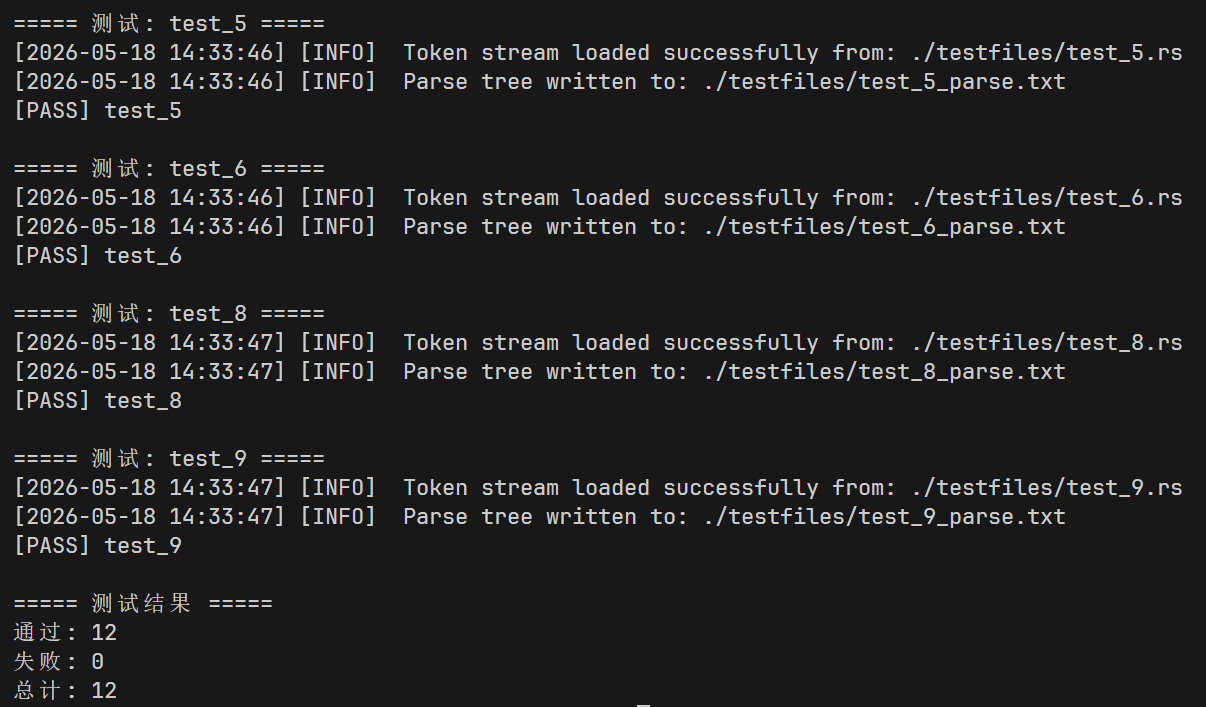
\includegraphics[width=\textwidth]{figures/cli_screenshot.png}
    \caption{命令行批量测试运行截图（12 个测试全部通过）}
\end{figure}

\begin{figure}[H]
    \centering
    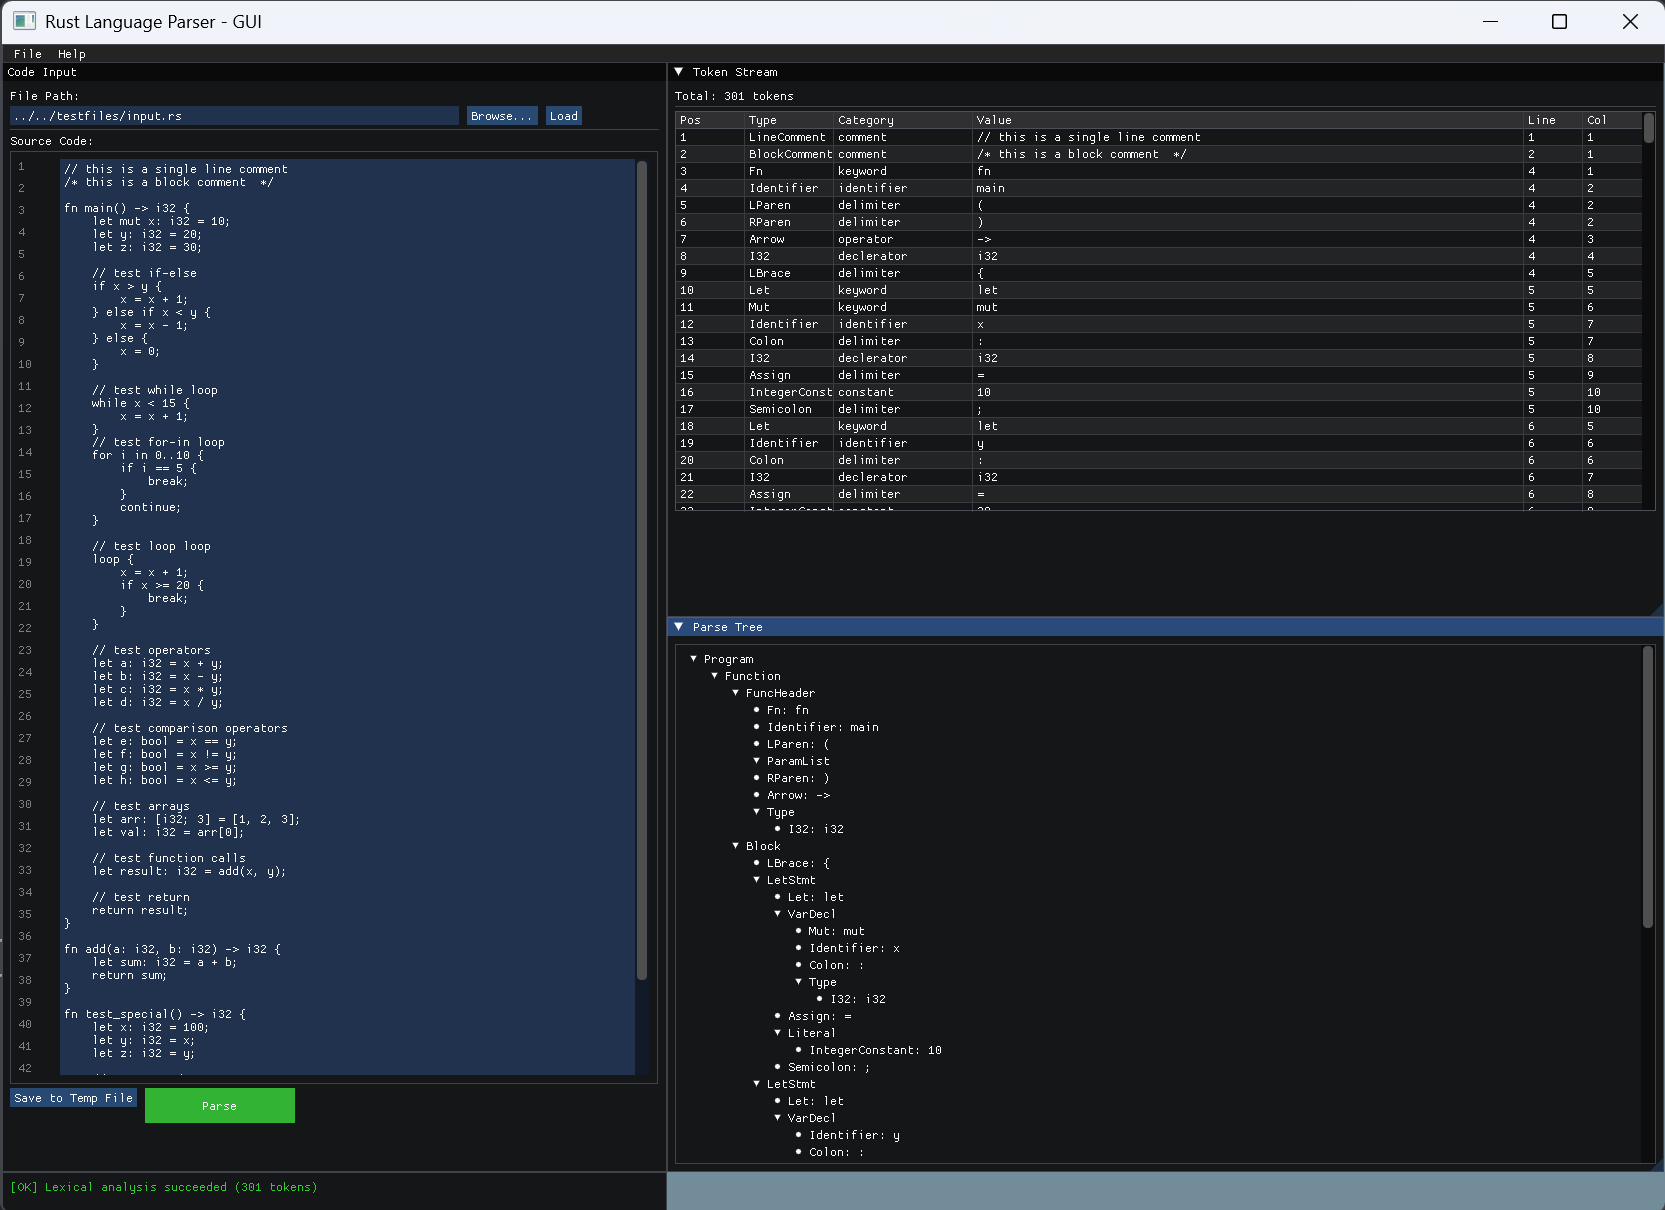
\includegraphics[width=\textwidth]{figures/gui_screenshot.png}
    \caption{GUI 界面运行截图：代码输入、Token 表格与语法树可视化}
\end{figure}

\newpage

% ============================================================
%  第八章 思考与分析
% ============================================================
\section{思考与分析}

作业最后提出了两个思考题，本节分别进行分析和讨论。

\subsection{思考题一：1.4 函数输入中的形参列表可以识别怎样的语言？}

规则 1.4 定义了函数形参列表的文法：

\begin{align}
\langle\text{形参列表}\rangle &\rightarrow \epsilon \mid \langle\text{形参}\rangle \mid \langle\text{形参}\rangle \ \texttt{,} \ \langle\text{形参列表}\rangle \\
\langle\text{形参}\rangle &\rightarrow \langle\text{变量属性}\rangle \ \texttt{ID} \ \texttt{:} \ \langle\text{类型}\rangle
\end{align}

其中 $\langle\text{变量属性}\rangle$ 由规则 0.1 和 6.1 定义为 \texttt{mut} 或 $\epsilon$，$\langle\text{类型}\rangle$ 由规则 0.2 定义为 \texttt{i32}（后续扩展规则增加数组类型、引用类型、元组类型等）。

\textbf{语言描述。}该文法生成的语言为：零个或多个形参组成的逗号分隔列表，每个形参由可选的 \texttt{mut} 修饰符、标识符、冒号和类型组成。用正则表达式可描述为：

$$L(\langle\text{形参列表}\rangle) = \epsilon \mid P(\texttt{,} \ P)^{*}$$

其中 $P = \texttt{[mut] ID : Type}$。合法的形参列表举例如下：

\begin{lstlisting}[language=RustLike]
fn f()                  // 空
fn f(a: i32)            // 单参数
fn f(mut a: i32, b: i32)  // 多参数
fn f(a: i32, mut b: i32, c: i32)  // 任意长度
\end{lstlisting}

\textbf{形式语言分析。}从形式语言的角度，该文法虽然是上下文无关文法（2 型），但其递归结构仅用于生成逗号分隔的列表，等价于正则表达式 $\epsilon \mid P(\texttt{,}P)^*$，因此 $\langle\text{形参列表}\rangle$ 定义的语言实际上是一个\textbf{正则语言}（3 型）。这是因为递归仅出现在产生式的最右端（右递归），没有嵌套结构。

\textbf{LL(1) 分析。}该文法满足 LL(1) 条件：对于 $\langle\text{形参列表}\rangle$ 的三条候选产生式，可以通过查看第一个输入符号做出唯一选择：
\begin{itemize}
    \item 若当前符号为 \texttt{)}，选择 $\epsilon$（空形参列表）
    \item 若当前符号为 \texttt{Mut} 或 \texttt{Identifier}，选择包含 $\langle\text{形参}\rangle$ 的产生式
    \item 进入 $\langle\text{形参}\rangle$ 后，由后续是否出现 \texttt{,} 决定是否继续递归
\end{itemize}

因此，该文法可以被递归下降分析器直接处理，无需回溯。

\subsection{思考题二：9.1 元组比 8.1 数组多了几条产生式，为什么？}

\textbf{数量对比。}

规则 8.1 数组类型新增 \textbf{1 条}产生式：
\begin{align}
\langle\text{类型}\rangle &\rightarrow \texttt{[} \ \langle\text{类型}\rangle \ \texttt{;} \ \texttt{NUM} \ \texttt{]}
\end{align}

规则 9.1 元组类型新增 \textbf{3 条}产生式：
\begin{align}
\langle\text{类型}\rangle &\rightarrow \texttt{(} \ \langle\text{元组类型内部}\rangle \ \texttt{)} \\
\langle\text{元组类型内部}\rangle &\rightarrow \epsilon \mid \langle\text{类型}\rangle \ \texttt{,} \ \langle\text{类型列表}\rangle \\
\langle\text{类型列表}\rangle &\rightarrow \epsilon \mid \langle\text{类型}\rangle \mid \langle\text{类型}\rangle \ \texttt{,} \ \langle\text{类型列表}\rangle
\end{align}

因此，元组类型比数组类型多 \textbf{2 条}产生式（3 vs 1）。

\textbf{原因分析。}

\begin{enumerate}
    \item \textbf{数组元素类型单一（同构）}：数组 $[\texttt{T}; \texttt{N}]$ 中所有元素共享同一类型 \texttt{T}，数量由常量 \texttt{N} 确定。因此只需一条产生式，将"元素类型"和"长度"两个信息固定在方括号内即可完整描述。

    \item \textbf{元组元素类型各异（异构）}：元组 $(\texttt{T}_1, \texttt{T}_2, \ldots, \texttt{T}_n)$ 中每个位置可以是不同的类型，必须逐一枚举每个位置的独立类型。这需要：
    \begin{itemize}
        \item 一条产生式定义元组类型的括号结构
        \item 一条产生式处理元组内部（含空元组即单元类型 \texttt{()}）
        \item 一条产生式递归处理类型列表
    \end{itemize}

    \item \textbf{空元组的特殊处理}：元组允许空形式 $\texttt{()}$（单元类型），需要在 $\langle\text{元组类型内部}\rangle$ 中提供 $\epsilon$ 候选。而数组即使长度为 0 也写作 $[\texttt{T}; 0]$，结构固定，无需特殊处理。

    \item \textbf{本质差异}：数组类型的描述是"一个类型 $\times$ 一个数量"的固定模式；元组类型的描述是"任意多个可能不同的类型的序列"，属于列表结构，需要递归产生式来处理不定长的类型枚举。
\end{enumerate}

简言之，数组的\textbf{同构性}使其文法天然简洁（一条产生式足够），而元组的\textbf{异构性}要求更复杂的文法来逐一描述每个位置的类型（需要三条产生式）。

\subsection{部分羁绊分析}

作业最后指出了若干条文法规则之间的\textbf{羁绊}关系——这些约束超越了纯粹的语法结构，属于\textbf{语义层面}的要求。当前的词法分析和语法分析器仅完成前端编译器的语法部分，尚未实现语义分析，因此以下约束在现有系统中不做检测。本节分析每条羁绊的含义及其在语义分析阶段应有的处理方式。

\subsubsection{羁绊一：赋值语句 + 类型规则——类型不匹配应报错}

规则 2.2 定义了赋值语句 $\langle\text{赋值语句}\rangle \rightarrow \langle\text{左值}\rangle \ \texttt{=} \ \langle\text{表达式}\rangle \ \texttt{;}$，而规则 8.1 等拓展了 $\langle\text{类型}\rangle$，使其不再局限于 \texttt{i32}，还包含数组类型 $[\texttt{T}; \texttt{N}]$、引用类型 $\texttt{\&T}$ 等。

\textbf{语义约束：}当变量声明时指定了类型 \texttt{T}，后续赋值的表达式类型也应为 \texttt{T}（或可隐式转换为 \texttt{T}）。例如：

\begin{lstlisting}[language=RustLike]
let a: i32 = 42;        // OK: i32 <- i32
let b: [i32; 3] = [1, 2, 3]; // OK: [i32;3] <- [i32;3]
let c: i32 = [1, 2, 3]; // ERROR: i32 <- [i32;3]
\end{lstlisting}

\textbf{实现思路：}需要在语法分析之后引入\textbf{类型检查}（Type Checking）阶段。为每个表达式节点标注类型，沿语法树自底向上传播类型信息，在赋值节点处比较左值类型与右值类型是否一致。

\subsubsection{羁绊二：for 循环 + 数组——仅数组为可迭代结构}

规则 5.2 定义了 for 循环：$\langle\text{for语句}\rangle \rightarrow \texttt{for} \ \langle\text{变量声明}\rangle \ \texttt{in} \ \langle\text{可迭代结构}\rangle \ \langle\text{语句块}\rangle$。规则 8.2 拓展了 $\langle\text{可迭代结构}\rangle$，使其可以是数组。

\textbf{语义约束：}for-in 循环的迭代目标必须是可迭代结构。在当前文法中，可迭代结构包括范围表达式 \texttt{start..end} 和数组。其他类型的变量（如 \texttt{i32}）不可迭代，应报错。例如：

\begin{lstlisting}[language=RustLike]
for mut i in 0..10 { }      // OK: 范围是可迭代的
let arr: [i32; 3] = [1, 2, 3];
for mut x in arr { }         // OK: 数组是可迭代的
let a: i32 = 42;
for mut x in a { }           // ERROR: i32 不可迭代
\end{lstlisting}

\textbf{实现思路：}在语义分析阶段，检查 for-in 循环中 $\langle\text{可迭代结构}\rangle$ 的类型。若为范围类型或数组类型则合法，否则报错。这需要维护一个\textbf{符号表}（Symbol Table），记录每个变量的类型信息。

\subsubsection{羁绊三：赋值语句 + 变量不可变属性——对不可变变量赋值应报错}

规则 6.1 拓展了 $\langle\text{变量属性}\rangle \rightarrow \epsilon$，即变量可以声明为不可变（不加 \texttt{mut}）。规则 2.2 和循环规则（5.2 等）中可能存在对不可变变量的赋值。

\textbf{语义约束：}不可变变量只能被声明和读取，不能被重新赋值。例如：

\begin{lstlisting}[language=RustLike]
let a: i32 = 1;
a = 2;                       // ERROR: a 不可变，不能赋值

let mut b: i32 = 1;
b = 2;                       // OK: b 是可变变量

for mut i in 0..10 {
    i = 5;                    // OK: i 声明为 mut
}
\end{lstlisting}

\textbf{实现思路：}在符号表中为每个变量记录其\textbf{可变性}（mutability）属性。在遇到赋值语句时，查询左值对应的变量是否为 \texttt{mut}，若不是则报错。

\textbf{总结。}上述三条羁绊均属于语义约束，需要引入\textbf{符号表}和\textbf{类型系统}才能在编译阶段检测。当前实现聚焦于词法分析和语法分析，语义分析作为后续改进方向。完整的编译器应在语法树构建完成后，遍历语法树进行语义检查（类型检查、可变性检查等），确保程序的语义正确性。

\subsection{LR(1) 冲突分析}

作业鼓励思考文法中是否存在 LR(1) 无法处理的情况。本节分析类 Rust 文法中的潜在冲突。

\subsubsection{经典悬空 else 问题}

在许多语言中，if-else 语句存在悬空 else（dangling else）歧义：

\begin{lstlisting}[language=RustLike]
if a > 0 then if b > 0 then x = 1 else x = 2
// else 匹配内层 if 还是外层 if？
\end{lstlisting}

然而，\textbf{本项目的文法不存在悬空 else 问题}。因为规则 4.1 使用 $\langle\text{语句块}\rangle$（即 \texttt{\{...\}}）作为 if 和 else 的体，而非 $\langle\text{语句}\rangle$。花括号明确界定了每个块的范围，消除了歧义：

\begin{lstlisting}[language=RustLike]
if a > 0 {
    if b > 0 { ... }
} else {
    ...
}
// else 始终匹配外层 if，因为内层 if 已被 {} 包围
\end{lstlisting}

\subsubsection{规则 7.0 中的移进-归约冲突}

规则 7.0 定义了函数表达式语句串：

\begin{align}
\langle\text{函数表达式语句串}\rangle &\rightarrow \langle\text{表达式}\rangle \mid \langle\text{语句}\rangle \ \langle\text{函数表达式语句串}\rangle
\end{align}

而 $\langle\text{语句}\rangle$ 的候选包含 $\langle\text{表达式}\rangle \ \texttt{;}$（规则 3.1 的表达式语句）。因此，当分析器在块内解析了一个 $\langle\text{表达式}\rangle$ 后，面对下一个符号 \texttt{;} 时：

\begin{itemize}
    \item \textbf{归约（Reduce）}：将 $\langle\text{表达式}\rangle$ 直接归约为 $\langle\text{函数表达式语句串}\rangle$，将其视为\textbf{尾表达式}（block 的返回值）
    \item \textbf{移进（Shift）}：移进 \texttt{;}，与 $\langle\text{表达式}\rangle$ 一起归约为 $\langle\text{语句}\rangle$，然后继续解析后续内容
\end{itemize}

这构成了一个经典的\textbf{移进-归约冲突}（Shift-Reduce Conflict）。例如以下代码：

\begin{lstlisting}[language=RustLike]
let mut z = {
    let mut t = x * x + x;
    t = t + x * y;
    t           // <-- 此处是尾表达式还是表达式语句？
};
\end{lstlisting}

在解析到 `t` 之后，若下一个符号是 `;`，分析器不知道 `t` 是尾表达式（使整个块返回 `t` 的值）还是需要移进 `;` 构成表达式语句 `t;`。

\textbf{产生原因：}产生式 $\langle\text{函数表达式语句串}\rangle \rightarrow \langle\text{表达式}\rangle$ 和 $\langle\text{语句}\rangle \rightarrow \langle\text{表达式}\rangle \ \texttt{;}$ 共享了前缀 $\langle\text{表达式}\rangle$，且区分符号 \texttt{;} 出现在 $\langle\text{表达式}\rangle$ 之后而非之前，因此仅凭一个向前查看符号无法在归约点做出决策。

\textbf{解决方案——改写产生式。}可以将函数表达式语句串改写为\textbf{显式分离}语句部分和尾表达式部分：

\begin{align}
\langle\text{函数表达式语句块}\rangle &\rightarrow \texttt{\{} \ \langle\text{语句列表}\rangle \ [\langle\text{表达式}\rangle] \ \texttt{\}} \\
\langle\text{语句列表}\rangle &\rightarrow \epsilon \mid \langle\text{语句}\rangle \ \langle\text{语句列表}\rangle
\end{align}

改写后，$\langle\text{语句列表}\rangle$ 中只包含以 \texttt{;} 结尾的语句，而 $\langle\text{表达式}\rangle$ 作为可选的尾表达式出现在语句列表之后。决策规则清晰：
\begin{itemize}
    \item 若当前符号为 \texttt{\}}，且之前有语句，则语句列表结束，无尾表达式
    \item 若当前符号为表达式的起始（\texttt{ID}、\texttt{NUM}、\texttt{(} 等），解析 $\langle\text{表达式}\rangle$，然后检查下一个符号：
    \begin{itemize}
        \item 若为 \texttt{;}，则这是一个表达式语句，归入 $\langle\text{语句列表}\rangle$
        \item 若为 \texttt{\}}，则这是一个尾表达式
    \end{itemize}
\end{itemize}

这种改写完全消除了移进-归约冲突，且与 Rust 语言的实际语义一致：块内先执行语句，最后一个不带分号的表达式作为块的返回值。

\textbf{为什么原始文法难以在 LR(1) 中处理。}根本原因在于 $\langle\text{函数表达式语句串}\rangle$ 的两条候选产生式以同一非终结符 $\langle\text{表达式}\rangle$ 开头，而区分信息（\texttt{;} vs \texttt{\}}）出现在 $\langle\text{表达式}\rangle$ \textbf{之后}。LR(1) 的向前查看符号位于归约点，此时 $\langle\text{表达式}\rangle$ 已被归约，但 \texttt{;} 尚未被消耗——分析器必须在"将已归约的 $\langle\text{表达式}\rangle$ 作为尾表达式"和"继续移进 \texttt{;} 构成语句"之间做选择。改写后的文法通过引入 $\langle\text{语句列表}\rangle$ 将判断推迟到消耗 \texttt{;} 之后，从而解决了冲突。

\subsubsection{其他潜在冲突分析}

\textbf{元组表达式 vs 括号表达式（规则 3.1、9.2）：}规则 3.1 中 $\langle\text{因子}\rangle \rightarrow \texttt{(} \ \langle\text{表达式}\rangle \ \texttt{)}$ 与规则 9.2 中 $\langle\text{可取元素}\rangle \rightarrow \texttt{(} \ \langle\text{元组赋值内部}\rangle \ \texttt{)}$ 均以 \texttt{(} 开头。但在 LR(1) 中，解析完第一个表达式后，下一个符号是 \texttt{)} 还是 \texttt{,} 可以明确区分两者：\texttt{)} 对应括号表达式，\texttt{,} 对应元组表达式。因此\textbf{不构成 LR(1) 冲突}。

\textbf{乘法 vs 解引用（规则 3.4、6.4）：}运算符 \texttt{*} 同时出现在乘法表达式 $\langle\text{项}\rangle \rightarrow \langle\text{项}\rangle \ \texttt{*} \ \langle\text{因子}\rangle$ 和解引用表达式 $\langle\text{左值}\rangle \rightarrow \texttt{*} \ \langle\text{左值}\rangle$ 中。但在 LR(1) 中，上下文可以明确区分：若 \texttt{*} 出现在二元运算符位置（前一个符号是因子/表达式），则为乘法；若出现在一元位置（前一个符号是语句开头或另一个运算符），则为解引用。\textbf{不构成 LR(1) 冲突}。

\textbf{数组下标 vs 数组字面量（规则 8.2、8.3）：}\texttt{[} 既可以开始数组字面量 $\texttt{[} \ \langle\text{数组元素列表}\rangle \ \texttt{]}$，也可以开始数组下标 $\langle\text{可取元素}\rangle \ \texttt{[} \ \langle\text{表达式}\rangle \ \texttt{]}$。但前者出现在因子（表达式起始）位置，后者出现在已有可取元素之后，上下文不同。\textbf{不构成 LR(1) 冲突}。

\newpage

% ============================================================
%  第九章 总结与反思
% ============================================================
\section{总结与反思}

\subsection{项目成果总结}

本项目成功实现了类Rust语言的前端编译器，主要成果包括：

\begin{enumerate}
    \item \textbf{词法分析器}：基于Flex实现，能够正确识别关键字、运算符、界符、常量、标识符、注释等词法单元
    \item \textbf{语法分析器}：采用递归下降分析法，能够正确解析函数定义、控制流语句、表达式等语法结构
    \item \textbf{语法树生成}：实现了清晰的语法树数据结构和输出格式
    \item \textbf{可视化界面}：基于ImGui实现了直观的GUI展示
    \item \textbf{跨平台支持}：支持Linux和Windows双平台编译运行
\end{enumerate}

\subsection{遇到的问题与解决方案}

在项目开发过程中，我们遇到了以下主要问题：

\begin{enumerate}
    \item \textbf{正则表达式优先级问题}

    问题：关键字和标识符的正则表达式可能冲突，如\texttt{let}可能被识别为标识符。

    解决方案：在Flex规则中将关键字规则置于标识符规则之前，Flex按规则顺序优先匹配。

    \item \textbf{左递归问题}

    问题：表达式文法存在左递归，无法直接用于递归下降分析。

    解决方案：采用消除左递归的标准方法，将文法改写为分层结构，并通过循环结构处理连续运算符。

    \item \textbf{运算符优先级处理}

    问题：如何正确处理多层级运算符优先级。

    解决方案：采用分层解析方法，每层函数对应一个优先级，通过函数调用层次确保高优先级运算符先被处理。

    \item \textbf{跨平台编译问题}

    问题：Windows平台缺少GLFW等依赖库。

    解决方案：使用vcpkg进行跨平台依赖管理，在Linux上使用MinGW-w64进行交叉编译。

    \item \textbf{特殊字符处理}

    问题：字符串常量中的换行符影响输出格式。

    解决方案：设计自定义转义规则，将特殊字符转换为可识别的转义序列。
\end{enumerate}

\subsection{知识收获与能力提升}

通过本次项目实践，我们获得了以下收获：

\begin{enumerate}
    \item \textbf{理论知识深化}：深入理解了词法分析（有限状态自动机）和语法分析（递归下降）的理论基础
    \item \textbf{工程实践能力}：掌握了Flex工具的使用、CMake构建系统配置、跨平台编译技术
    \item \textbf{代码设计能力}：学习了语法树数据结构设计、流式接口设计等软件设计方法
    \item \textbf{团队协作经验}：通过分工合作，提升了项目管理和团队协作能力
\end{enumerate}

\subsection{改进方向与展望}

项目仍有改进空间，主要包括：

\begin{enumerate}
    \item \textbf{错误恢复机制}：当前语法分析器遇到错误即停止，可改进为错误恢复后继续分析
    \item \textbf{更多语法特性}：可扩展支持结构体、枚举、泛型等复杂语法
    \item \textbf{语义分析阶段}：实现类型检查、作用域分析等语义分析功能
    \item \textbf{代码生成阶段}：生成中间代码或目标代码，完成完整编译流程
    \item \textbf{性能优化}：优化词法分析的Token缓冲机制，提升大文件处理效率
\end{enumerate}

\subsection{个人想法与体会}

\subsubsection{对文法设计的见解}

本次作业的文法设计呈现出一种\textbf{渐进式拓展}的风格：从最简单的空函数（1.1）开始，逐步添加语句、表达式、控制流、引用、数组、元组等特性。每条新规则都明确标注了所依赖的前置规则和被拓展的规则，构成了一张清晰的\textbf{依赖图}。这种设计方法给我们两点启发：

\begin{enumerate}
    \item \textbf{文法可以增量式构建}。在实际的编译器开发中，往往也需要从核心语言开始，逐步添加特性。这种分层次的文法组织方式不仅便于学习理解，也便于分阶段实现和测试。我们的项目正是按此思路推进：先确保必选规则（0.1--5.1）全部通过，再逐步实现扩展规则。

    \item \textbf{产生式之间存在非平凡的交互}。如"部分羁绊分析"中讨论的，不同规则之间的组合可能引入语义层面的约束（类型检查、可变性检查），这些约束在单独看某条规则时并不明显，只有在组合使用时才会暴露。这说明编译器设计不能只关注单条文法规则，还必须考虑规则之间的全局交互。
\end{enumerate}

此外，我们注意到文法中 $\langle\text{可取元素}\rangle$ 和 $\langle\text{可取引用}\rangle$ 的设计有其巧妙之处：通过将"可以出现在赋值号左侧"的结构统一为一个非终结符，文法自然地描述了 Rust 中\textbf{所有权和借用}体系的语法基础。例如，规则 6.2--6.4 通过为 $\langle\text{可取引用}\rangle$ 添加 `\&` 和 `\& mut` 候选，在语法层面就区分了可变引用和不可变引用。

\subsubsection{对实现方案的取舍思考}

在项目实现过程中，我们做出了若干设计取舍：

\textbf{递归下降 vs 工具生成。}语法分析器选择了手写递归下降而非使用 Yacc/Bison 等工具生成。手写递归下降的优势在于：
\begin{itemize}
    \item \textbf{错误信息质量高}：可以在每个解析函数中提供精确的上下文信息（如"解析函数参数时期望标识符"），而工具生成的分析器往往只能给出"syntax error"
    \item \textbf{控制力强}：可以灵活处理特殊的语法结构，如 \texttt{parseExprOrAssignStmt()} 先解析表达式再判断是否为赋值，避免了将赋值和表达式分为不同入口的复杂性
    \item \textbf{易于调试}：每个解析函数对应一个非终结符，可以单独设置断点、打印日志
\end{itemize}

代价是需要手动消除左递归和管理运算符优先级。我们采用经典的分层解析方法（每层函数对应一个优先级），虽然代码量稍多，但逻辑清晰、易于维护。

\textbf{TokenStream 流式接口 vs 数组加载。}我们选择将词法分析结果全部加载到内存中的 \texttt{vector<Token>}，而非逐 token 喂给语法分析器。这简化了实现（语法分析器可以随时向前查看任意位置），但对于超大文件可能会有内存压力。在实际编译器中（如 GCC、LLVM），通常采用按需读取+缓冲的策略，在内存效率和灵活性之间取得平衡。

\textbf{注释过滤策略。}我们选择在词法分析阶段生成注释 Token，但在语法分析之前统一过滤（\texttt{remove\_comments()}），而非在词法分析阶段直接跳过。这样做的好处是保留了注释信息，可以在 GUI 中展示完整的 Token 流（包括注释），增强了可视化效果。这是一种以少量内存开销换取更好用户体验的权衡。

\subsubsection{对 Rust 语言特性的分析}

通过实现类 Rust 语言的编译器前端，我们对 Rust 的语法设计有了更深入的理解：

\textbf{显式类型声明}。Rust 要求在函数参数和大部分变量声明中显式标注类型（虽然支持局部类型推导），这与我们文法中 $\langle\text{形参}\rangle \rightarrow \langle\text{变量属性}\rangle \ \texttt{ID} \ \texttt{:} \ \langle\text{类型}\rangle$ 的设计一致。显式类型使语法分析更简单——不需要复杂的类型推导机制，仅在语法分析阶段就能获取完整的类型信息。

\textbf{块即表达式}。规则 7.0--7.4 揭示了 Rust 的一个核心设计哲学：\textbf{几乎一切皆是表达式}。花括号块可以求值，if-else 可以求值，loop 也可以求值。这使得 Rust 不需要三元运算符 \texttt{? :}，因为 \texttt{if-else} 本身就是表达式。虽然在本次项目中由于实现复杂度暂未支持这一特性，但这种"表达式导向"的设计理念对我们有深刻启发——它使语言的语法更加统一和正交。

\textbf{可变性显式标注}。Rust 的 \texttt{mut} 关键字要求程序员显式声明变量的可变性，默认不可变。这一设计在文法中体现为 $\langle\text{变量属性}\rangle \rightarrow \texttt{mut} \mid \epsilon$（规则 0.1 和 6.1）。从编译器的角度看，\texttt{mut} 不仅是语法糖，更是一种语义承诺：编译器可以基于可变性信息进行更激进的优化（如不可变变量的值可以被缓存）。同时，它也使得\textbf{别名+可变性}的检查成为可能，这正是 Rust 借用检查器（Borrow Checker）的核心工作。

\textbf{运算符的多义性}。项目中 \texttt{*} 同时表示乘法和解引用，\texttt{\&} 同时表示按位与和取地址（引用）。在语法层面，这些可以通过上下文区分（二元位置 vs 一元位置），但在语义层面，Rust 进一步利用类型信息消歧——这种"语法相同但语义不同"的设计在编程语言中并不少见，它要求语义分析阶段有足够的类型信息才能做出正确判断。

\newpage

% ============================================================
%  参考文献
% ============================================================
\section{参考文献}

\begin{enumerate}
    \item Rust 程序设计语言中文版. \url{https://rustwiki.org/zh-CN/book/}
    \item 自己动手写编译器. \url{https://pandolia.net/tinyc/index.html}
    \item 北京大学编译实践课程在线文档. \url{https://pku-minic.github.io/online-doc/}
    \item antlr/grammars-v4: Grammars written for ANTLR v4. \url{https://github.com/antlr/grammars-v4}
    \item CLIUtils/CLI11: Command line parser for C++11. \url{https://github.com/CLIUtils/CLI11}
    \item ocornut/imgui: Dear ImGui. \url{https://github.com/ocornut/imgui}
    \item Flex手册. \url{https://westes.github.io/flex/manual/}
    \item Alfred V. Aho, Monica S. Lam, Ravi Sethi, Jeffrey D. Ullman. 编译原理（第2版）. 机械工业出版社.
\end{enumerate}

\newpage

% ============================================================
%  附录A：完整文法规则列表
% ============================================================
\section*{附录A\quad 完整文法规则列表}
\addcontentsline{toc}{section}{附录A\quad 完整文法规则列表}
\markboth{附录A\quad 完整文法规则列表}{附录A\quad 完整文法规则列表}
\renewcommand{\thesubsection}{A.\arabic{subsection}}
\setcounter{subsection}{0}

\subsection{完整产生式列表}

{\allowdisplaybreaks
\begin{align}
&\textbf{程序结构} \\
Program &\rightarrow FunctionList \\
FunctionList &\rightarrow Function \mid Function \ FunctionList \\
Function &\rightarrow FuncHeader \ Block \\
FuncHeader &\rightarrow \texttt{fn} \ Identifier \ \texttt{(} \ ParamList \ \texttt{)} \ [\texttt{->} \ Type] \\
ParamList &\rightarrow \epsilon \mid Param \mid Param \ \texttt{,} \ ParamList \\
Param &\rightarrow [\texttt{mut}] \ Identifier \ \texttt{:} \ Type \\
Block &\rightarrow \texttt{\{} \ StmtList \ \texttt{\}} \\
StmtList &\rightarrow \epsilon \mid Stmt \ StmtList \\
\\
&\textbf{语句} \\
Stmt &\rightarrow EmptyStmt \mid LetStmt \mid ReturnStmt \mid IfStmt \\
     &\quad\mid WhileStmt \mid ForStmt \mid LoopStmt \mid BreakStmt \\
     &\quad\mid ContinueStmt \mid Block \mid AssignStmt \mid ExprStmt \\
EmptyStmt &\rightarrow \texttt{;} \\
LetStmt &\rightarrow \texttt{let} \ VarDecl \ [\texttt{=} \ Expr] \ \texttt{;} \\
VarDecl &\rightarrow [\texttt{mut}] \ Identifier \ [\texttt{:} \ Type] \\
ReturnStmt &\rightarrow \texttt{return} \ [Expr] \ \texttt{;} \\
AssignStmt &\rightarrow LValue \ \texttt{=} \ Expr \ \texttt{;} \\
ExprStmt &\rightarrow Expr \ \texttt{;} \\
BreakStmt &\rightarrow \texttt{break} \ \texttt{;} \\
ContinueStmt &\rightarrow \texttt{continue} \ \texttt{;} \\
\\
&\textbf{控制流} \\
IfStmt &\rightarrow \texttt{if} \ Expr \ Block \ [ElseClause] \\
ElseClause &\rightarrow \texttt{else} \ Block \mid \texttt{else} \ IfStmt \\
WhileStmt &\rightarrow \texttt{while} \ Expr \ Block \\
ForStmt &\rightarrow \texttt{for} \ [\texttt{mut}] \ Identifier \ \texttt{in} \ Expr \ Block \\
LoopStmt &\rightarrow \texttt{loop} \ Block \\
\\
&\textbf{表达式（消除左递归后）} \\
Expr &\rightarrow RangeExpr \\
RangeExpr &\rightarrow CmpExpr \mid CmpExpr \ \texttt{..} \ CmpExpr \\
CmpExpr &\rightarrow AddExpr \mid CmpExpr \ CmpOp \ AddExpr \\
CmpOp &\rightarrow \texttt{==} \mid \texttt{!=} \mid \texttt{>} \mid \texttt{>=} \mid \texttt{<} \mid \texttt{<=} \\
AddExpr &\rightarrow MulExpr \mid AddExpr \ AddOp \ MulExpr \\
AddOp &\rightarrow \texttt{+} \mid \texttt{-} \\
MulExpr &\rightarrow Unary \mid MulExpr \ MulOp \ Unary \\
MulOp &\rightarrow \texttt{*} \mid \texttt{/} \\
Unary &\rightarrow \texttt{\&} \ [\texttt{mut}] \ Unary \mid \texttt{*} \ Unary \mid Atom \\
Atom &\rightarrow Constant \mid \texttt{(} \ Expr \ \texttt{)} \mid ArrayLit \\
     &\quad\mid Identifier \ [CallExpr \mid IndexExpr] \\
CallExpr &\rightarrow \texttt{(} \ ArgList \ \texttt{)} \\
IndexExpr &\rightarrow \texttt{[} \ Expr \ \texttt{]} \\
ArgList &\rightarrow \epsilon \mid Expr \mid Expr \ \texttt{,} \ ArgList \\
ArrayLit &\rightarrow \texttt{[} \ ExprList \ \texttt{]} \\
ExprList &\rightarrow \epsilon \mid Expr \mid Expr \ \texttt{,} \ ExprList \\
\\
&\textbf{类型} \\
Type &\rightarrow \texttt{i32} \mid Identifier \\
     &\quad\mid \texttt{[} \ Type \ \texttt{;} \ Constant \ \texttt{]} \\
     &\quad\mid \texttt{\&} \ [\texttt{mut}] \ Type \\
     &\quad\mid \texttt{(} \ TypeList \ \texttt{)} \\
TypeList &\rightarrow \epsilon \mid Type \mid Type \ \texttt{,} \ TypeList
\end{align}
}

\newpage

% ============================================================
%  附录B：完整测试输入及输出
% ============================================================
\section*{附录B\quad 完整测试输入及输出}
\addcontentsline{toc}{section}{附录B\quad 完整测试输入及输出}
\markboth{附录B\quad 完整测试输入及输出}{附录B\quad 完整测试输入及输出}
\renewcommand{\thesubsection}{B.\arabic{subsection}}
\setcounter{subsection}{0}

\subsection{完整词法分析输出}

完整词法分析输出共包含约290个Token，详见项目文件\nolinkurl{parser/testfiles/lexer_output.tsv}。

\subsection{完整语法树输出}

完整语法树输出包含3个函数定义，共约480行，详见项目文件\nolinkurl{parser/testfiles/parse_tree.txt}。

\subsection{运行命令示例}

\begin{lstlisting}[language=bash, caption={命令行运行示例}]
# Linux
./parser --input input.rs --lexer-output lexer.tsv --parser-output tree.txt

# Windows
parser.exe --input input.rs --lexer-output lexer.tsv --parser-output tree.txt

# GUI模式（Windows）
parser.exe --gui --input input.rs
\end{lstlisting}

\end{document}